%% This is an example first chapter.  You should put chapter/appendix that you
%% write into a separate file, and add a line \include{yourfilename} to
%% main.tex, where `yourfilename.tex' is the name of the chapter/appendix file.
%% You can process specific files by typing their names in at the 
%% \files=
%% prompt when you run the file main.tex through LaTeX.
\chapter{The characterization of chimeric DNA rearrangements in single amplified human genomes across innovative single-cell technologies}
% \section{Abstract}
% We applied in-gel digital multiple displacement amplification (dMDA) to human cells and demonstrated whole-genome sequencing of single-cell MDA products with markedly reduced chimerism compared with 3 other recently developed single-cell technologies. 
\section{Introduction}
Transposable elements (TEs, `jumping genes') are discrete pieces of DNA that can move within the genome of a single cell and between the genomes of different cells. Nearly 45\% of the human genome is derived from TEs \cite{Perrat:2013cr,Cordaux:2009bb}. Studies have shown that TEs can cause mosaic copy-number variations (CNVs) and structural variations (SVs) on genes such as PIK3CA, AKT3 and mTOR during prenatal brain development. These mutations could result in brain malformation and neurological defects, including epilepsy, intellectual disability and hemimegalencephaly \cite{Lee:2014jp,Poduri:2013jp}. Thus, it is important to identify such mutation mechanisms and the affected diverse cell types that disrupt the function of the cortical circuits. In order to achieve this, targeted qPCR assay can be used to detect an increase in the copy number of TE. However, a critical limitation is that the genomic location of the new insertion cannot be identified \cite{Erwin:2014ir}. 

Single-cell targeted sequencing and whole genome sequencing approaches have enabled the location identification of novel brain-specific TE insertions. But the results are often confounded by the inherent false discovery rate of current technology \cite{Erwin:2014ir}. Single-cell technology has also been widely applied in several other scientific and biomedical field. For example, the screening of embryos using single-cell technologies on polar bodies and blastomeres has shown improved \textit{in vitro} fertilization success by eliminating embryos with a high frequency (30 $\times$ above baseline) of chromosomal rearrangements, which often lead to miscarriages \cite{Vanneste:2011dl}. This technique also lowers the rate of Mendelian disease through genome-wide single nucleotide variations (SNVs) screening on the embryos \cite{Hou:2013ub, Kuliev:2011jy}. 

% In order to understand the impact of TEs in brain development and in the genome mosaicism of neurons. 
% tions19,20,23,28. Many of these approaches are confounded by several factors, including the rarity of each individual insertion event (such events are likely to be hemizygous and present in a single cell or a subset of cells) and the inherent false discovery rate in next-generation sequenc- ing efforts. Nevertheless, several studies with varying levels of stringency have reported the identification of somatic insertions in the brain19,20,23,28

% Liquid biopsy has become increasingly prevalent in both clinical research and biotech ventures in diagnosing and monitoring patients with cancer, such as breast cancer and metastatic colorectal cancer. Liquid biopsy relies on single-cell techniques to detect a very low amount of partial or whole genomes of circulating tumor cells in the blood sample. The single-cell technologies mentioned above are desired to have a wide range of capabilities, such as contamination resistance, the ability to screen for rare targets, and an ideal trade-off between data quality and required hardware equipment support. However, current single-cell technologies don't satisfy most of the capabilities mentioned. 

% Need to define chimera functionally from Linda 

\begin{figure}
\centering
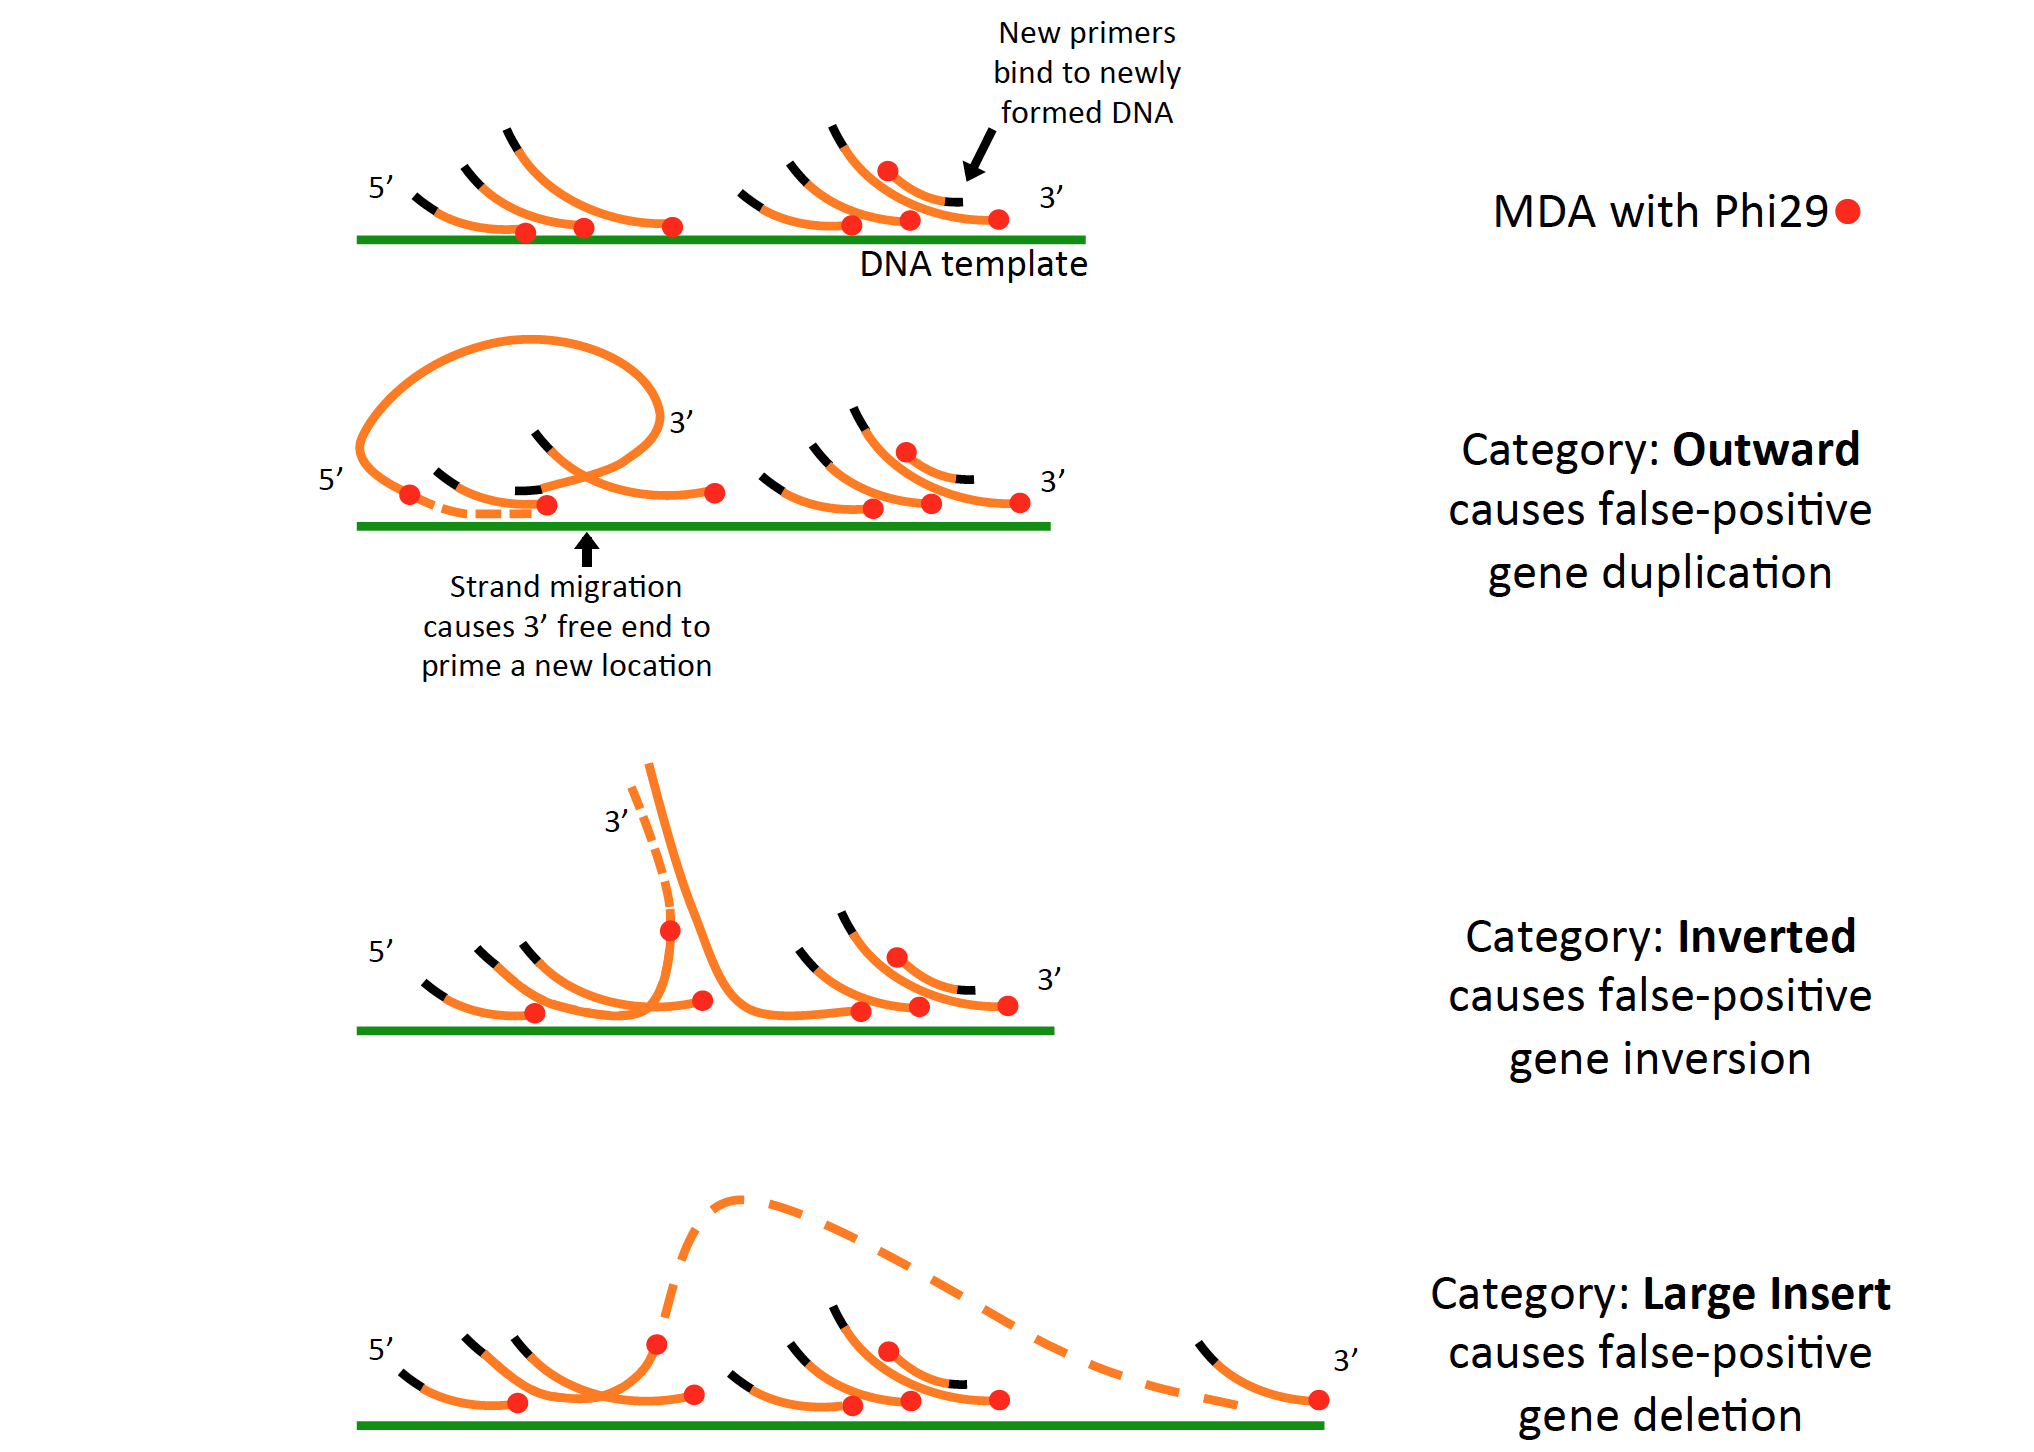
\includegraphics[keepaspectratio,width=1\textwidth]{./figures/ChimeraMechanism}
\caption[The mechanism of MDA chimera]{The mechanism of MDA chimera. The strand displacement action of MDA is shown on top. The strand migration dynamic causes the 3' end to freely bind to another part of the genome, resulting in outward, inverted and large-insert chimera. Cross-chromosome chimera is not shown but the mechanism is similar.}
\label{fig:chimeraMech}
\end{figure}

The data quality of single amplified and sequenced cells is a key to providing accurate and trustworthy information for above-mentioned applications. During the genome amplification and library preparation steps, artifacts are often generated that confound the detection of genomic signatures and complicate data analysis. These artifacts are often due to the implementation of the multiple displacement amplification (MDA) reaction and PCR-based sequencing library preparation \cite{Lasken:2007db}. One type of artifact generated by MDA--chimeric DNA rearrangements (Fig. \ref{fig:chimeraMech}), caused by the highly branched DNA secondary structures with free 3' ends of single-strand DNA during the reaction \cite{Lasken:2007db}, has raised flags in several single-cell studies. It has been shown that the preimplantation genetic diagnosis guided by single-cell genomics can be affected by false-positive SNVs and structural variations from MDA chimera \cite{VanderAa:2013jz, Voet:2013hk}. Researchers using single neurons to study developmental disorders discovered the complication of the chimera artifacts in identifying novel retrotransposon L1 as the existence of the chimera caused false-positive identifications of structural variations \cite{Evrony:2016du, Evrony:2015it}. This is also a problem for environmental microbes that lack a closely related reference genome. But in this chapter, we focus on human cells.   

% Rodrigue \textit{et al.} looked into the \textit{de novo} assembly of single \textit{prochlorococcus} and found inaccurate assembly from MDA chimera \cite{Rodrigue:2009gc}. Uncharacterized microbes such as \textit{prochlorococcus} don't have a reliable reference genome and it is difficult to screen out DNA rearrangements even with long-range sequencing technologies. 

Experimentally, several studies have made attempts to reduce such chimera artifacts. It has been shown that nanoliter microfluidic device might generate less MDA chimera than microliter samples \cite{Marcy:2007il}. However, nanoliter to picoliter microfluidic devices often require clean-room fabrication and supporting pneumatic instruments, which makes it hard to implement for labs with limited resource and funding. Zhang \textit{et al.} used a combination of $\Phi$29 polymerase debranching, S1 nuclease digestion and DNA polymerase I nick translation to reduce the chimeric rate in the library preparation step for single microbes \cite{Zhang:2006hq}, but such methods do not directly affect the chimera generated during MDA reaction. A recent study by Picher \textit{et al.} used a modified $\Phi$29 enzyme for whole genome amplification but didn't show evidence of reduced chimera compared to using unmodified $\Phi$29 \cite{Picher:2016ki}. A novel single-cell technology that is highly accessible and provides high-quality data, especially on reducing the MDA chimera artifact, is greatly needed. 

Bioinformatically, the majority of single-cell studies have focused on characterizing coverage uniformity, CNVs, SNVs, purity and throughput metrics, but have often neglected to quantify the amount of artifacts generated from single-cell whole genome amplification process and sequencing library preparation steps that affect assay performance. There exist established bioinformatic tools designed to filter chimera artifacts from 16S PCR reactions (comparing the phylogenies of fragments) \cite{Edgar:2011gy, Haas:2011jg} and single-cell RNA-seq experiments (with the matching of unique molecular identifiers and cell barcodes) \cite{Dixit:2016ki}. However, existing tools are not designed for chimera characterization and filtering in single MDA-amplified human genomes. A detailed bioinformatic characterization of MDA chimeras is needed to evaluate single-cell technologies and datasets that have been developed and produced. 

\begin{table}
\caption{Single-cell technology comparisons for chimera analysis}
\label{tab:chimeraTechTable}
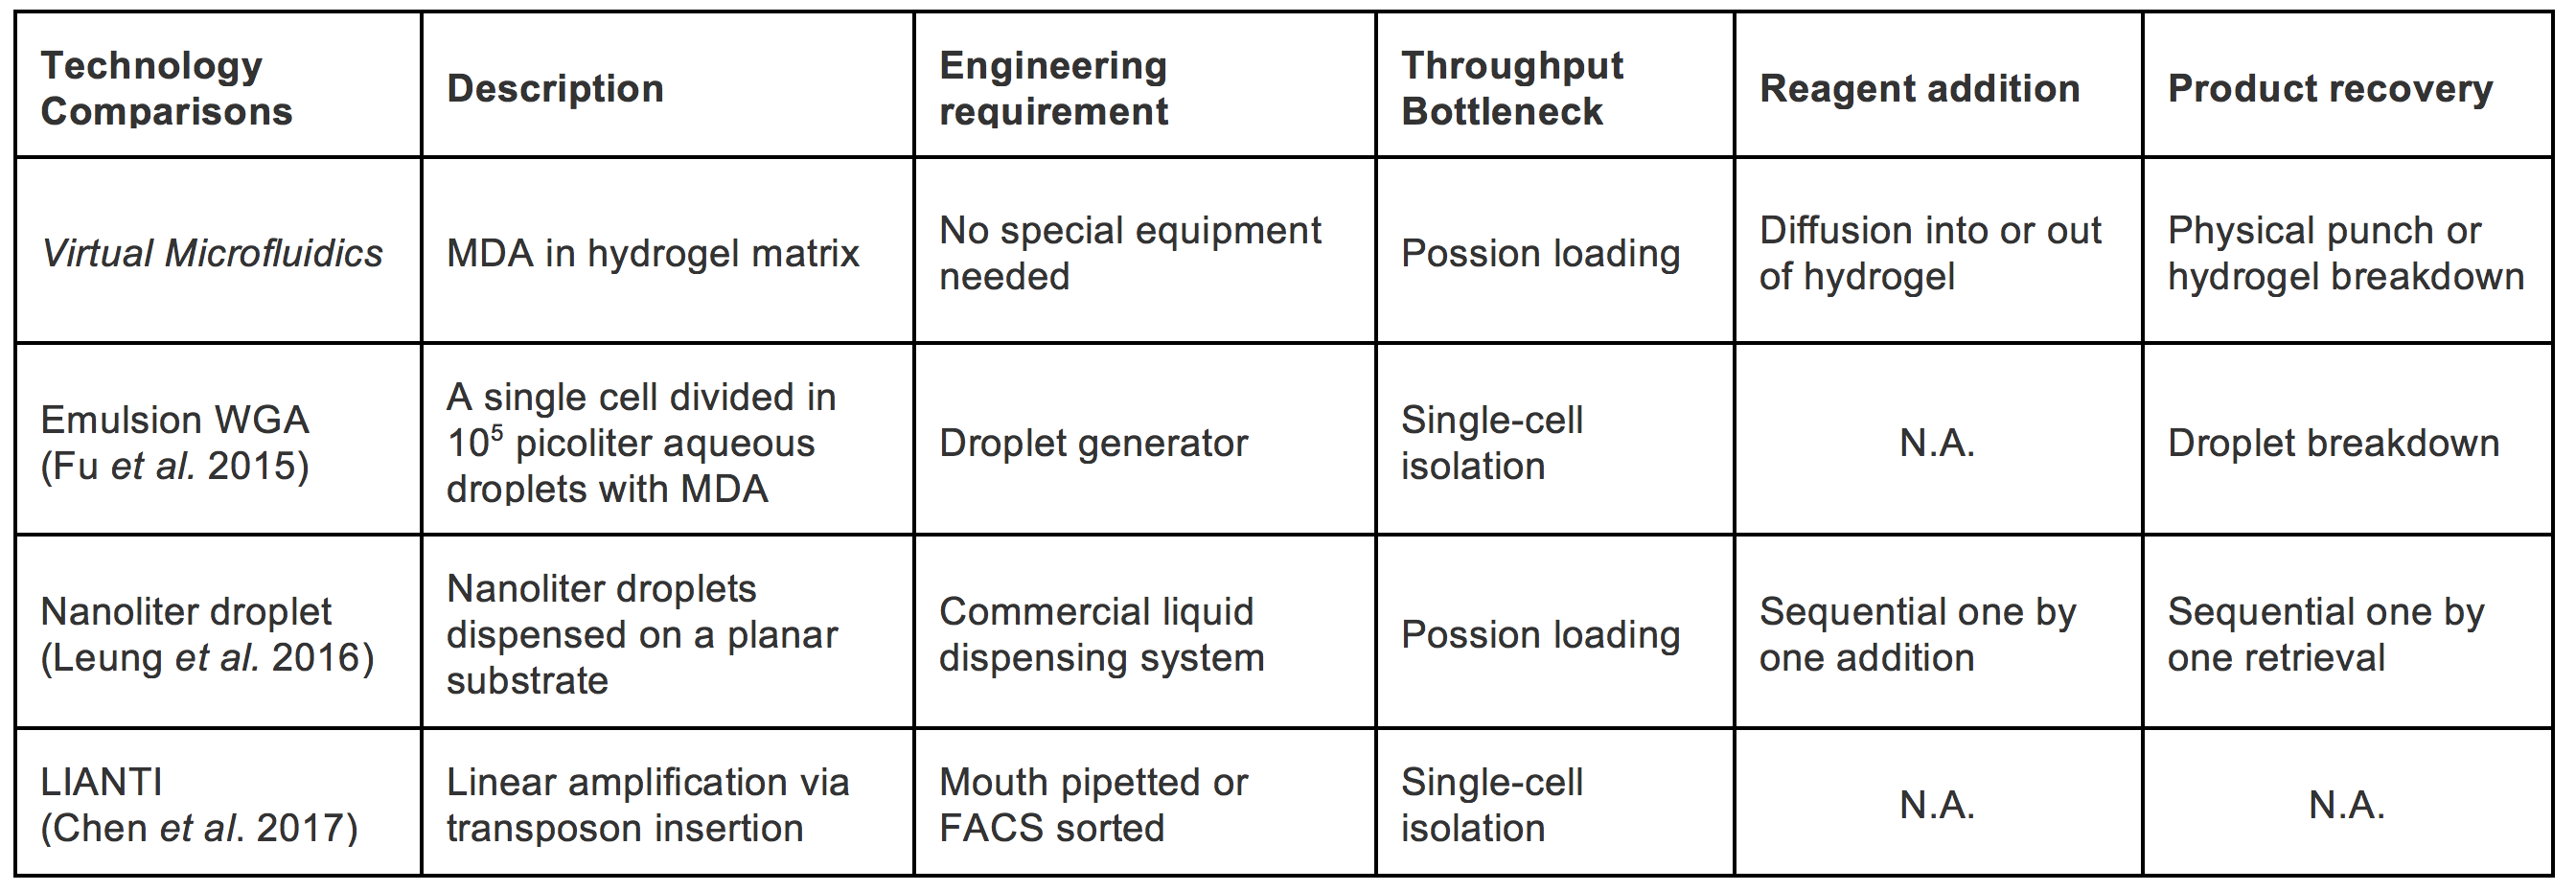
\includegraphics[width=\linewidth]{./figures/Chimera_TechTable}
\end{table}

In this study, we present the application of \textit{virtual microfluidics} on single human cells to demonstrate our technology's capabilities in producing high-quality single amplified human genomes with minimum equipment requirement. We benchmarked its performance with recent innovations of single-cell technologies (Table \ref{tab:chimeraTechTable}) based on exponential amplification method---MDA (eWGA, Nanodrop) and quasi-linear amplification method---LIANTI and MALBAC \cite{ Zong:2012bs,Fu:2015gl,Leung:2016vx,Chen:2017hq}. \textit{Virtual microfluidics} has been shown as a hydrogel-based single-cell isolation and amplification technology that is highly accessible and can provide high-quality single-cell whole genome amplification (WGA) product on cultured bacteria and human gut microbiome samples \cite{Xu:2016wt}. We have previously demonstrated its advantages on small genomes (bacteria) in terms of multi-fold chimera reduction and coverage uniformity improvement. Our hypothesis is that the single amplified human genomes in \textit{virtual microfluidics} will have a similar level of high-quality data to the previous study, with reduced chimeric DNA rearrangements and improved coverage uniformity. 

\begin{figure}
\centering
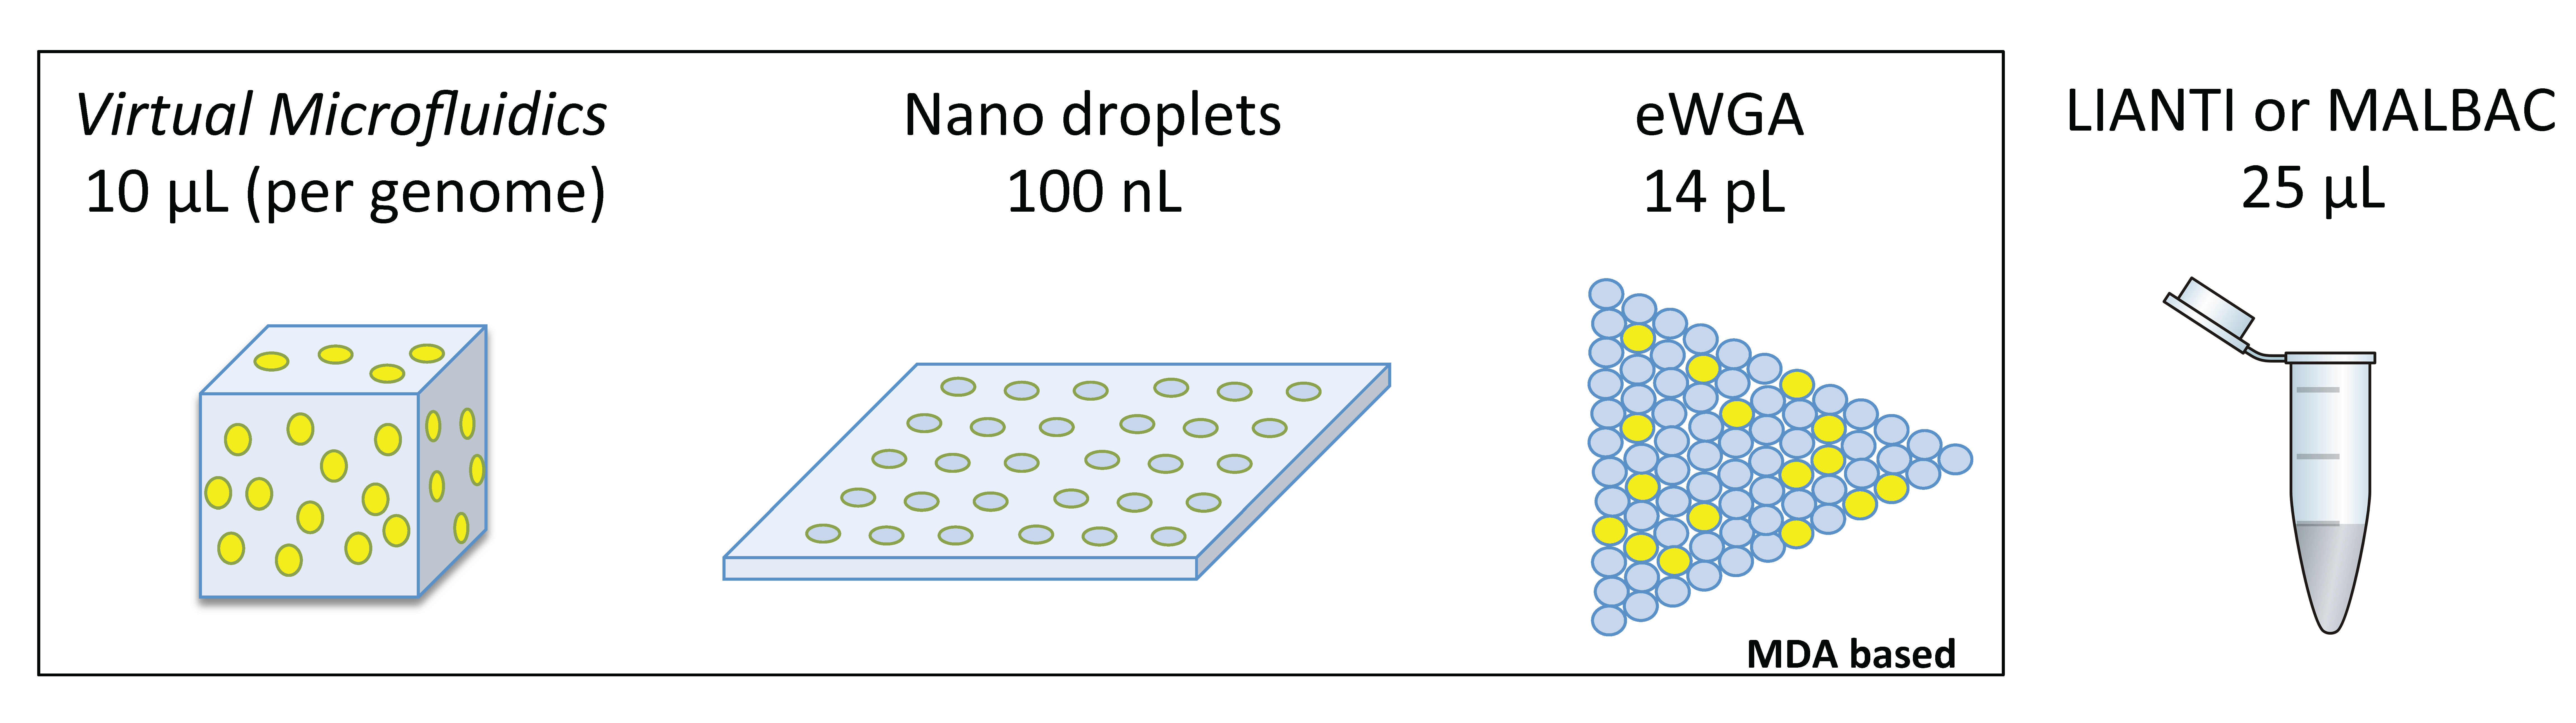
\includegraphics[keepaspectratio,width=1\textwidth]{./figures/Chimera_F1a_TechComparision.png}
\caption[Comparison of single-cell technologies]{Comparison of single-cell technologies. The volume labeled is for each single-cell genome amplification reaction.}
\label{fig:chimeraTech}
\end{figure}

As we mentioned in Chapter 3, the restricted diffusion of the MDA intermediates prevents cross-priming by isolating each portion of the product mixture. It limits cross-chromosome artifacts and chimera reads of large insert size (the distance between the forward read and reverse read mapped on the genome, $\Delta$ mapped coordinates + the length of reverse read). The hydrogel's micro-environment also physically limits the secondary DNA structures during MDA, thus reducing the chimera breakpoints out of total reads that are pair-mapped. To support the technology demonstration, we developed an algorithm to categorize the signatures of MDA chimeras across multiple single-cell platforms. This characterization will serve as a guidance for chimera analysis to be a non-negligible part of the analysis suite for evaluating future single-cell technologies.  

\section{Results and Discussion}
%%The discussion needs to draw comparative conclusions more directly (not just make qualitative general statements) from the data and describe the statistical support for these conclusions. The discussion should also tie back to the applications with some recommendations of what methods to use for which types of studies. There are still a number of typos and grammatical issues to clean up
We conducted modified \textit{virtual microfluidics} single-cell sequencing on 8 RPE--1 cells in a HiSeq 2500 lane with 2$\times$125 and obtained roughly 1$\times$ mapping depth to reference genome GRCh37-lite (methods). We characterized the single RPE cell dataset while benchmarking with unsorted\slash (unclear whether cherry-picked) single-cell datasets from eWGA (5 cells), MALBAC (2), tube MDA (2), Nanodrop (9) and LIANTI (3) (Table \ref{tab:chimeraDataSource}, Table \ref{tab:SRAaccession} and Fig. \ref{fig:chimeraTech}). All samples were trimmed and analyzed according to the analysis workflow (Fig. \ref{fig:chimeraWorkflow}). All mapped, de-duplicated, repeat-masked and sorted BAM files are down-sampled to 430,000 reads\slash sample ($\sim$0.01$\times$, including both forward and reverse reads) for chimera analysis (methods) . 

\begin{table}
\caption{Data source for chimera analysis}
\label{tab:chimeraDataSource}
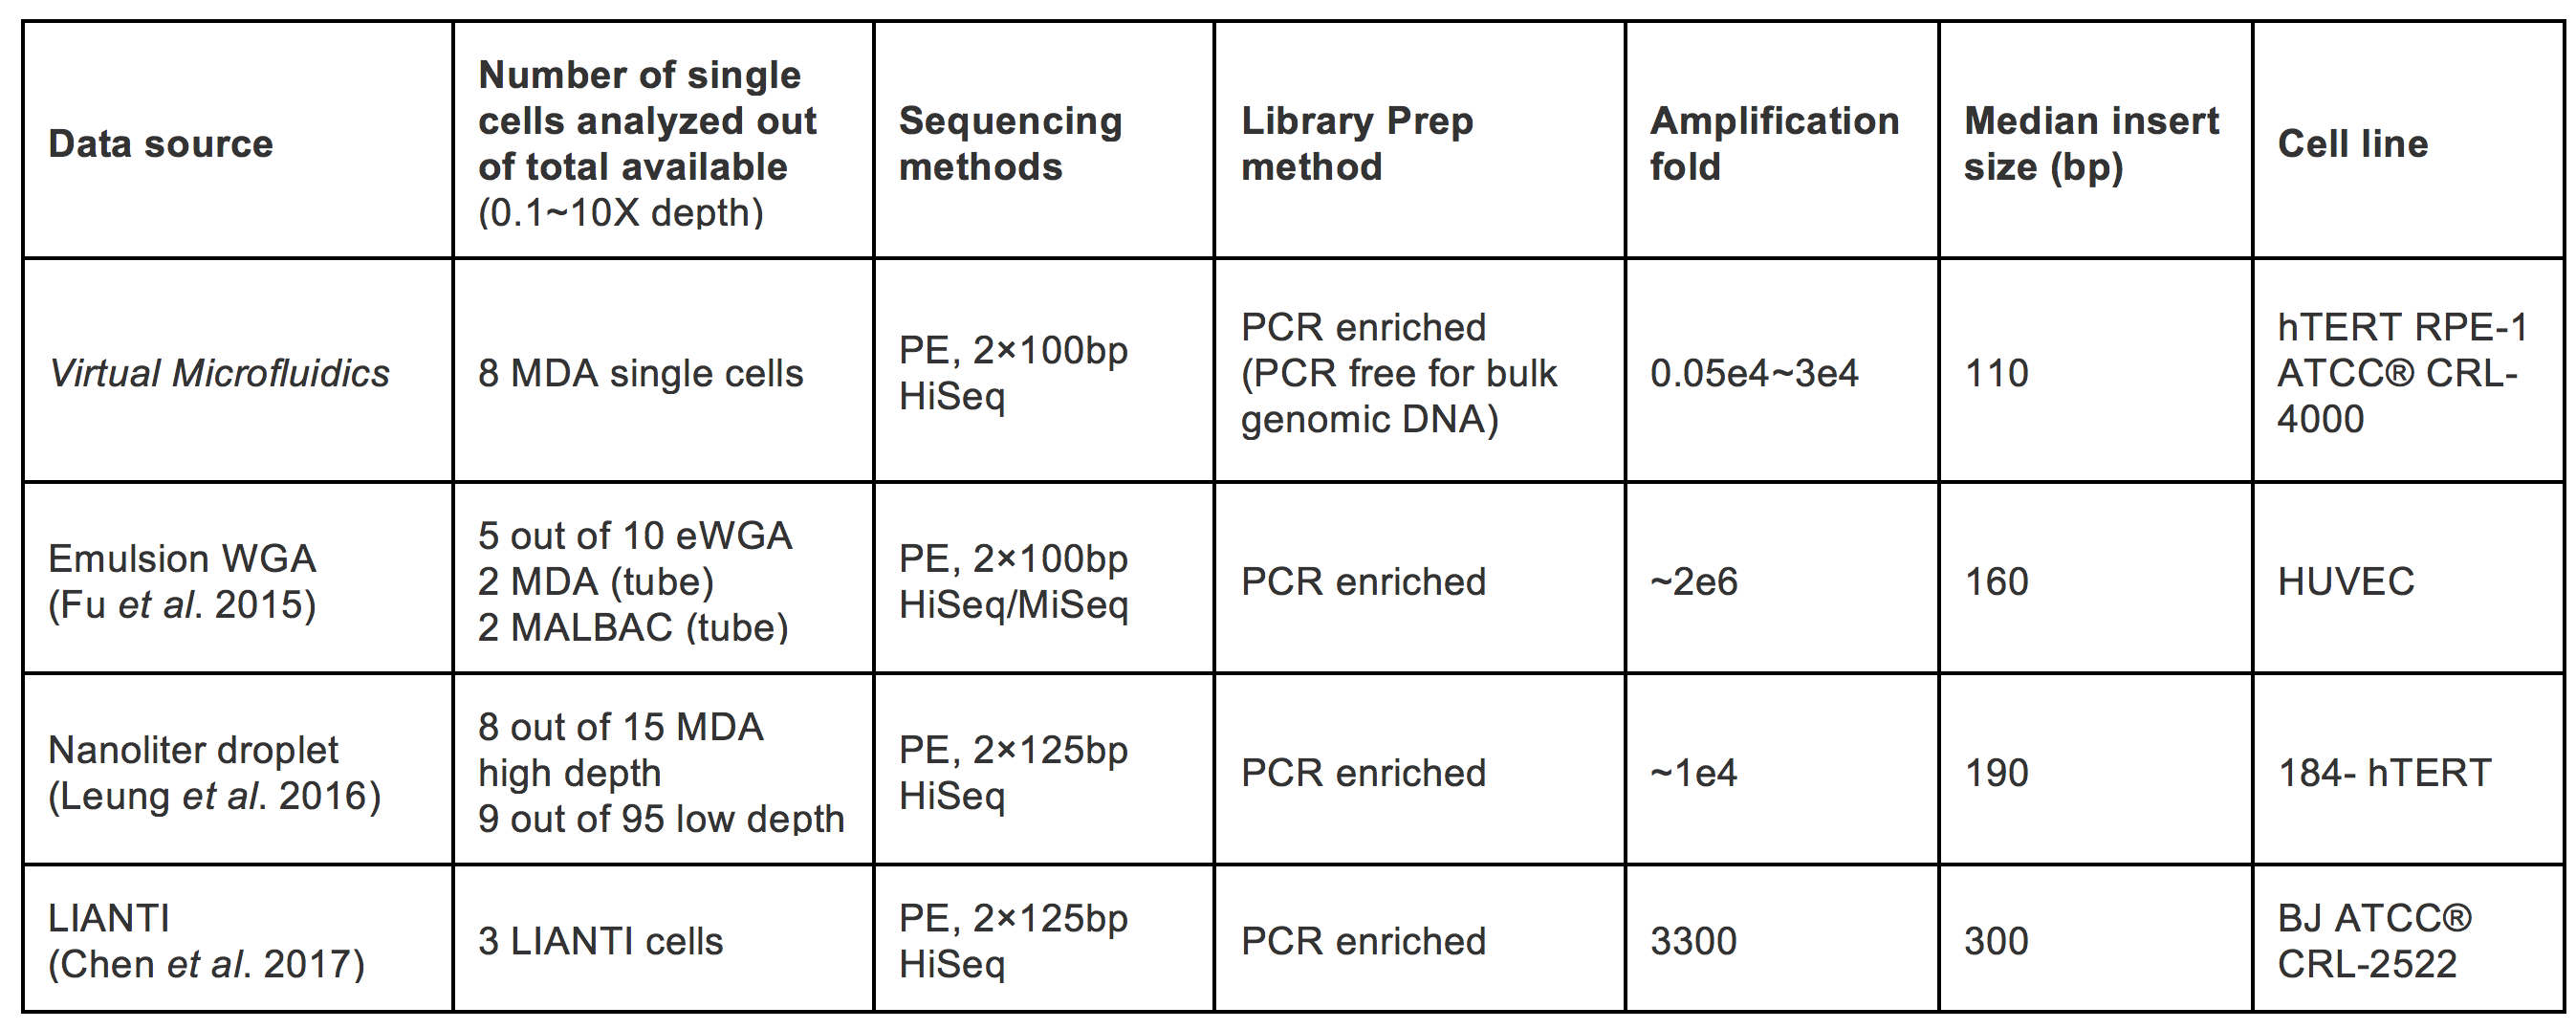
\includegraphics[width=\linewidth]{./figures/Chimera_DataTable}
\end{table}

The benchmarking datasets were chosen to represent different methods of cell isolation (hydrogel-based \textit{virtual microfluidics}, emulsion droplets, liquid dispensing), WGA chemistry (MDA, MALBAC, LIANTI) and library preparation methods (Nextera PCR-enriched and PCR-free ligation-based). According to Evrony \textit{et al.} 2015, most chimera originated from library preparation after MDA reaction. However, our previous study showed a multifold chimera rate reduction from MDA process in cultured bacteria compared to standard tube reactions using the same library preparation procedure (Nextera). Including above-mentioned datasets will help parse out the chimera characteristics and sources from single amplified human genomes. 

\begin{figure}
\centering
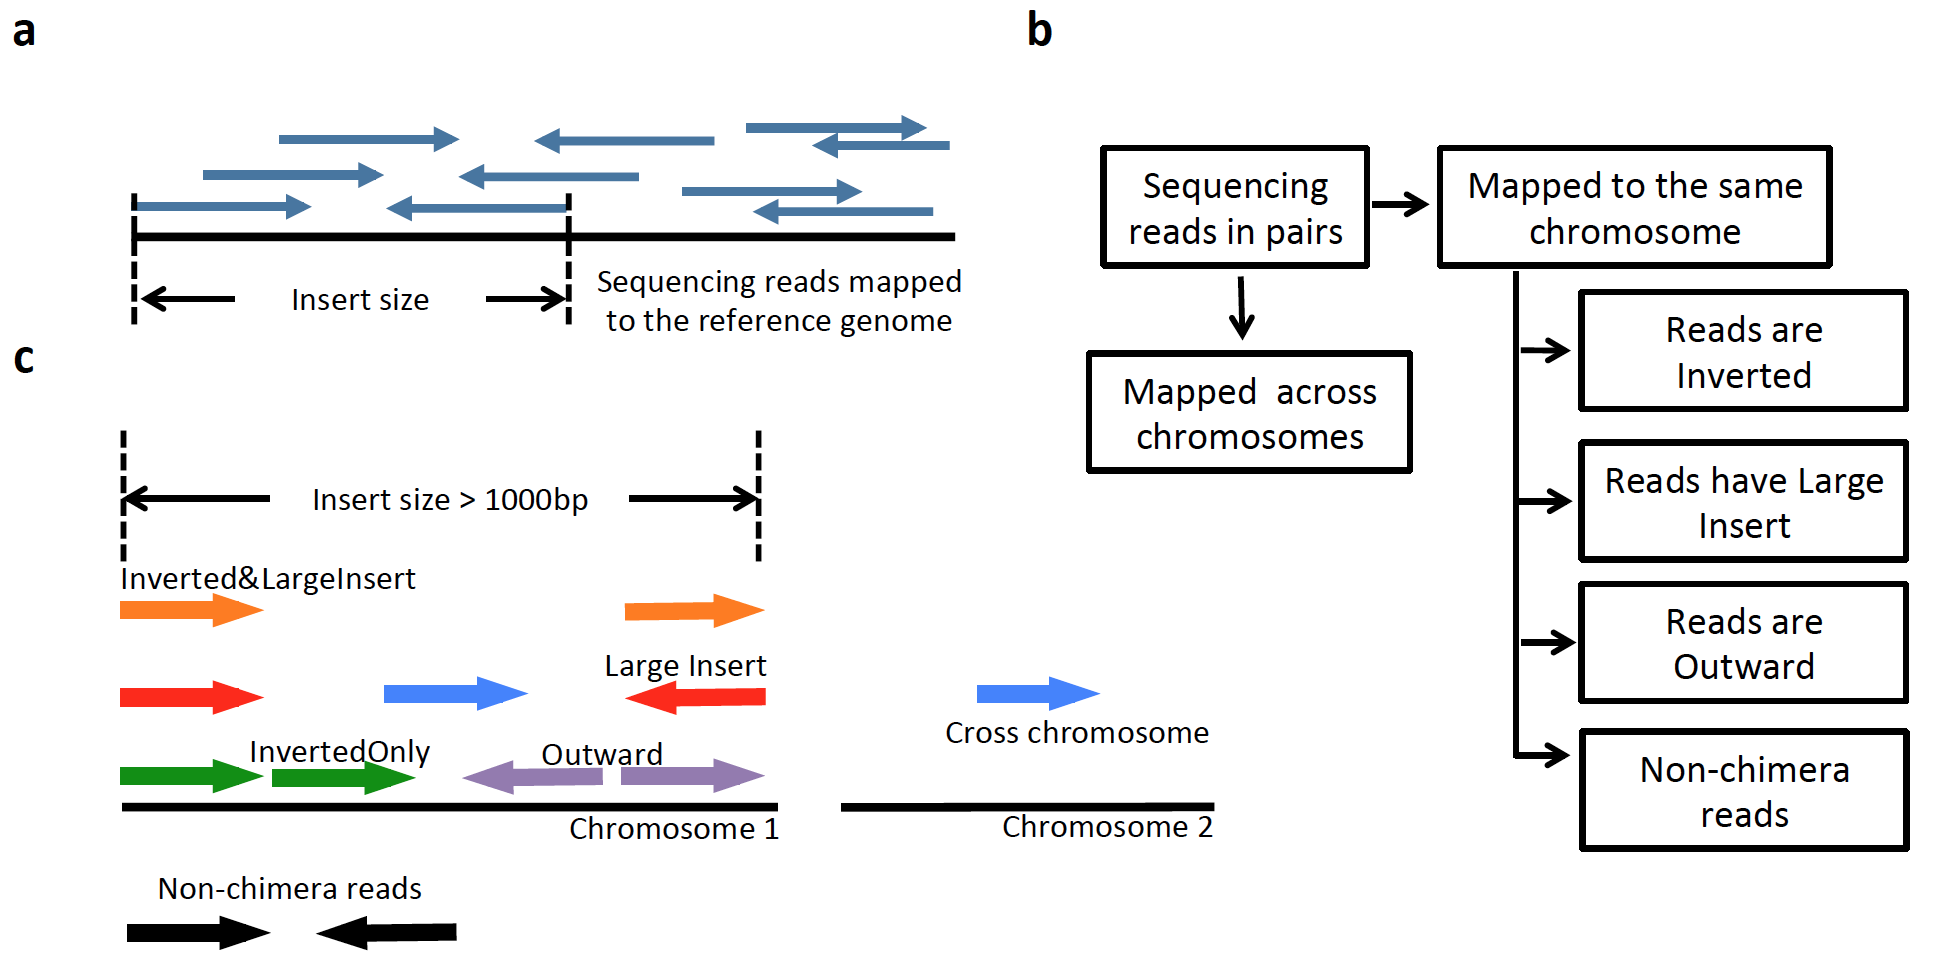
\includegraphics[keepaspectratio,width=1\textwidth]{./figures/ChimeraCategories_cropped}
\caption[Pair-ended sequencing for the chimera categorization.]{Pair-ended sequencing provides read orientations for the chimera categorization. (a) The insert size represents the length of DNA fragment. (b) The decision workflow to categorize different chimera reads. (c) Chimera and non-chimera reads are illustrated.}
\label{fig:chimeraWorkflow}
\end{figure}

It has been shown from a couple hundred sequencing reads of \textit{E. coli} that over 85\% of MDA chimeras are inverted read pairs, which means the forward and reverse read pairs don't have the correct orientation (inward facing) \cite{Lasken:2007db}. This type of sequencing result can be easily filtered out in a single-chromosome organism with the well-established reference genome, such as culturable bacteria. However, it becomes bioinformatically difficult when the reference genome is enriched with repeat islands in mammalian cells and when the draft genome is often inaccurate for unculturable environmental microbes. Making improvements in single-cell technologies is a task that needs to be done well both experimentally and bioinformatically. 

\subsection{Chimera categories}
A correct read pair should map to different strands (+/-, or sense and antisense) within the insert size range controlled by sequence library size selection (200 bp $\sim$ 800 bp). We defined five categories of chimera reads in this study (Fig. \ref{fig:chimeraWorkflow}b&c). Inverted means forward and reverse reads mapped to the same strand of DNA template (Fig. \ref{fig:chimeraWorkflow}c).  Within the inverted reads categories, the pairs of reads can be further categorized into inverted\&LargeInsert (>1000 bp insert size) and InvertedOnly (<1000 bp). For reads with the correct orientation, the pairs of reads can be categorized into LargeInsert Only chimera (>1000 bp) and cross-chromosome chimera. The color code in Fig. \ref{fig:chimeraWorkflow}c corresponds to the same categorizations in Fig. \ref{fig:chimera5Categories} chimera quantification. The five categories are mutually exclusive and collectively exhaustive for all chimeras that can be parsed out. 

\begin{figure}
\centering
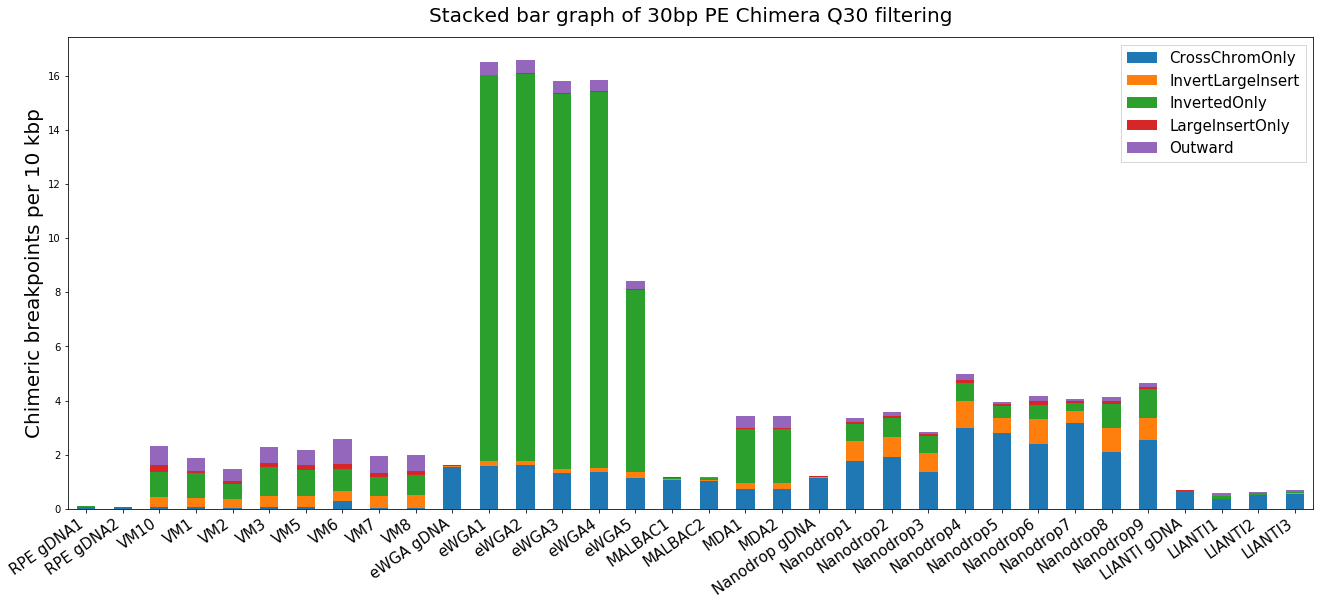
\includegraphics[keepaspectratio,width=1\textwidth]{./figures/20170727_ChimeraSubcategories_IScorrected_PE_30bp_Q30}
\caption[Chimeric breakpoints per 10 kbp]{Chimeric breakpoints per 10 kbp across all samples are shown as 5 categories of chimera: cross-chromosome, inverted, large insert size (>1000 bp), outward, and inverted large insert.}
\label{fig:chimera5Categories}
\end{figure}

The median insert size distribution of sequencing reads across different datasets varies from 100 bp $\sim$ 300 bp. In order to eliminate the factor of inconsistent insert size on chimera detection and possible read overlaps, we normalized the chimera breakpoints over total basepairs mapped and trimmed all sequencing reads to 30 bp \cite{Tu:2015dc}. Previous studies have revealed the nature of MDA chimera in terms of overlapping number of basepairs in the chimera junction \cite{Tu:2017fz, Tu:2015dc}. Here we focus on the categorization of MDA chimera in different single-cell whole genome amplification technologies on human cells and their genome-wide signatures. Single-ended and pair-ended mapping of the same sequencing dataset were implemented side by side to compare the read paring's impact on chimera detection. Here we define the chimera breakpoints as the total number of Read 1 and Read 2 that categorize as chimera reads (as there are two parts of the genome joined together, which represents two breakpoints). 

\begin{eqnarray*}
\text{Chimera breakpoints per 10 kbp} = \frac{ \text{Chimera reads } (R1 + R2) \times 10^4}{ \text{Total number of bp mapped}} \\
\\
= \frac{ \text{Chimera reads } (R1 + R2) \times 10^4}{ (\text{Total pairs of reads that are mapped}) \times \text{Average insert size}}
\end{eqnarray*}

Fig. \ref{fig:chimera5Categories} shows the number of chimeric breakpoints per 10 kbp mapped in a stacked bar graph. Genomic DNA (gDNA) samples without WGA serve as the baseline of comparisons. \textit{Virtual microfluidics} samples exhibit low chimera breakpoint frequency while confirming the 85\% inverted composition in MDA chimera. RPE gDNA was processed with PCR-free library preparation and is used as the negative control of chimera detection. The residual chimera detected from the RPE gDNA represents the inherent genome structural variations of the cell line. This also serves as the comparison for the chimera introduced by PCR library preparation process. The eWGA, Nanodrop, and LIANTI gDNA all went through PCR enrichment. But it is unknown whether these 3 cell lines used (PCR-free datasets unavailable) have inherently higher structural variations than RPE cell line does. 

Interestingly, the eWGA single cells show more than 90\% enrichment in \say{Inverted Only} chimera reads and a 3 $\sim$ 7 fold chimera frequency increase compared to the gDNA baseline. This increase can be explained by the isolation of individual fragments in picoliter liquid droplets. The confinement of a single DNA template in picoliter volume resulted in mostly inverted artifacts from MDA while few template was available for cross-chromosome priming to happen. The nanodrop dataset has a different pattern for chimera signature, showing more than 50\% chimeras that span across different chromosomes and 25\% chimeras with large insert size. Both eWGA and nanodrop methods have a higher frequency of chimera reads occurrence compared to microliter-ranged in-tube MDA. Our explanation is that a smaller reaction volume does not affect the secondary structure of a single-strand DNA. But a higher density of DNA increases the chance of cross priming. Due to the smaller reaction volume that increases the DNA density in the reaction, more chimeras are produced in eWGA and Nanodrop. 

%This finding contradicts to the previous study that claimed "nanoliter microfluidic device might generate less MDA chimera than microliter samples".

% \begin{figure}
% \begin{tabular}{lc}
% (a) \\
% \includegraphics[keepaspectratio,width=1\textwidth]{./figures/20170517_ChimericBreakpoint10kbp_PE_Qfiltered} \\
% (b) \\
% \includegraphics[keepaspectratio,width=1\textwidth]{./figures/20170517_ChimericBreakpoint10kbp_SE_Qfiltered} \\
% \end{tabular}
% \caption[The effect of mapping quality filtering on chimera detection.]{The effect of mapping quality filtering on chimera detection. (a) Pair-ended (PE) mapping with BWA aligner. (b) Single-ended (SE) mapping with BWA aligner}
% \label{fig:chimeraMappingQ}
% \end{figure}

\subsection{Chimera rate analysis with respect to mapping quality filtering} % (fold)
% subsection subsection_name (end)}
We implemented mapping quality filters (Q = 30, 20, 10) and found a slight decrease of chimera rate when increasing the mapping quality threshold as expected by the more stringent quality filtering (Fig. \ref{fig:chimeraMappingQAll}). 

\begin{figure}
\centering
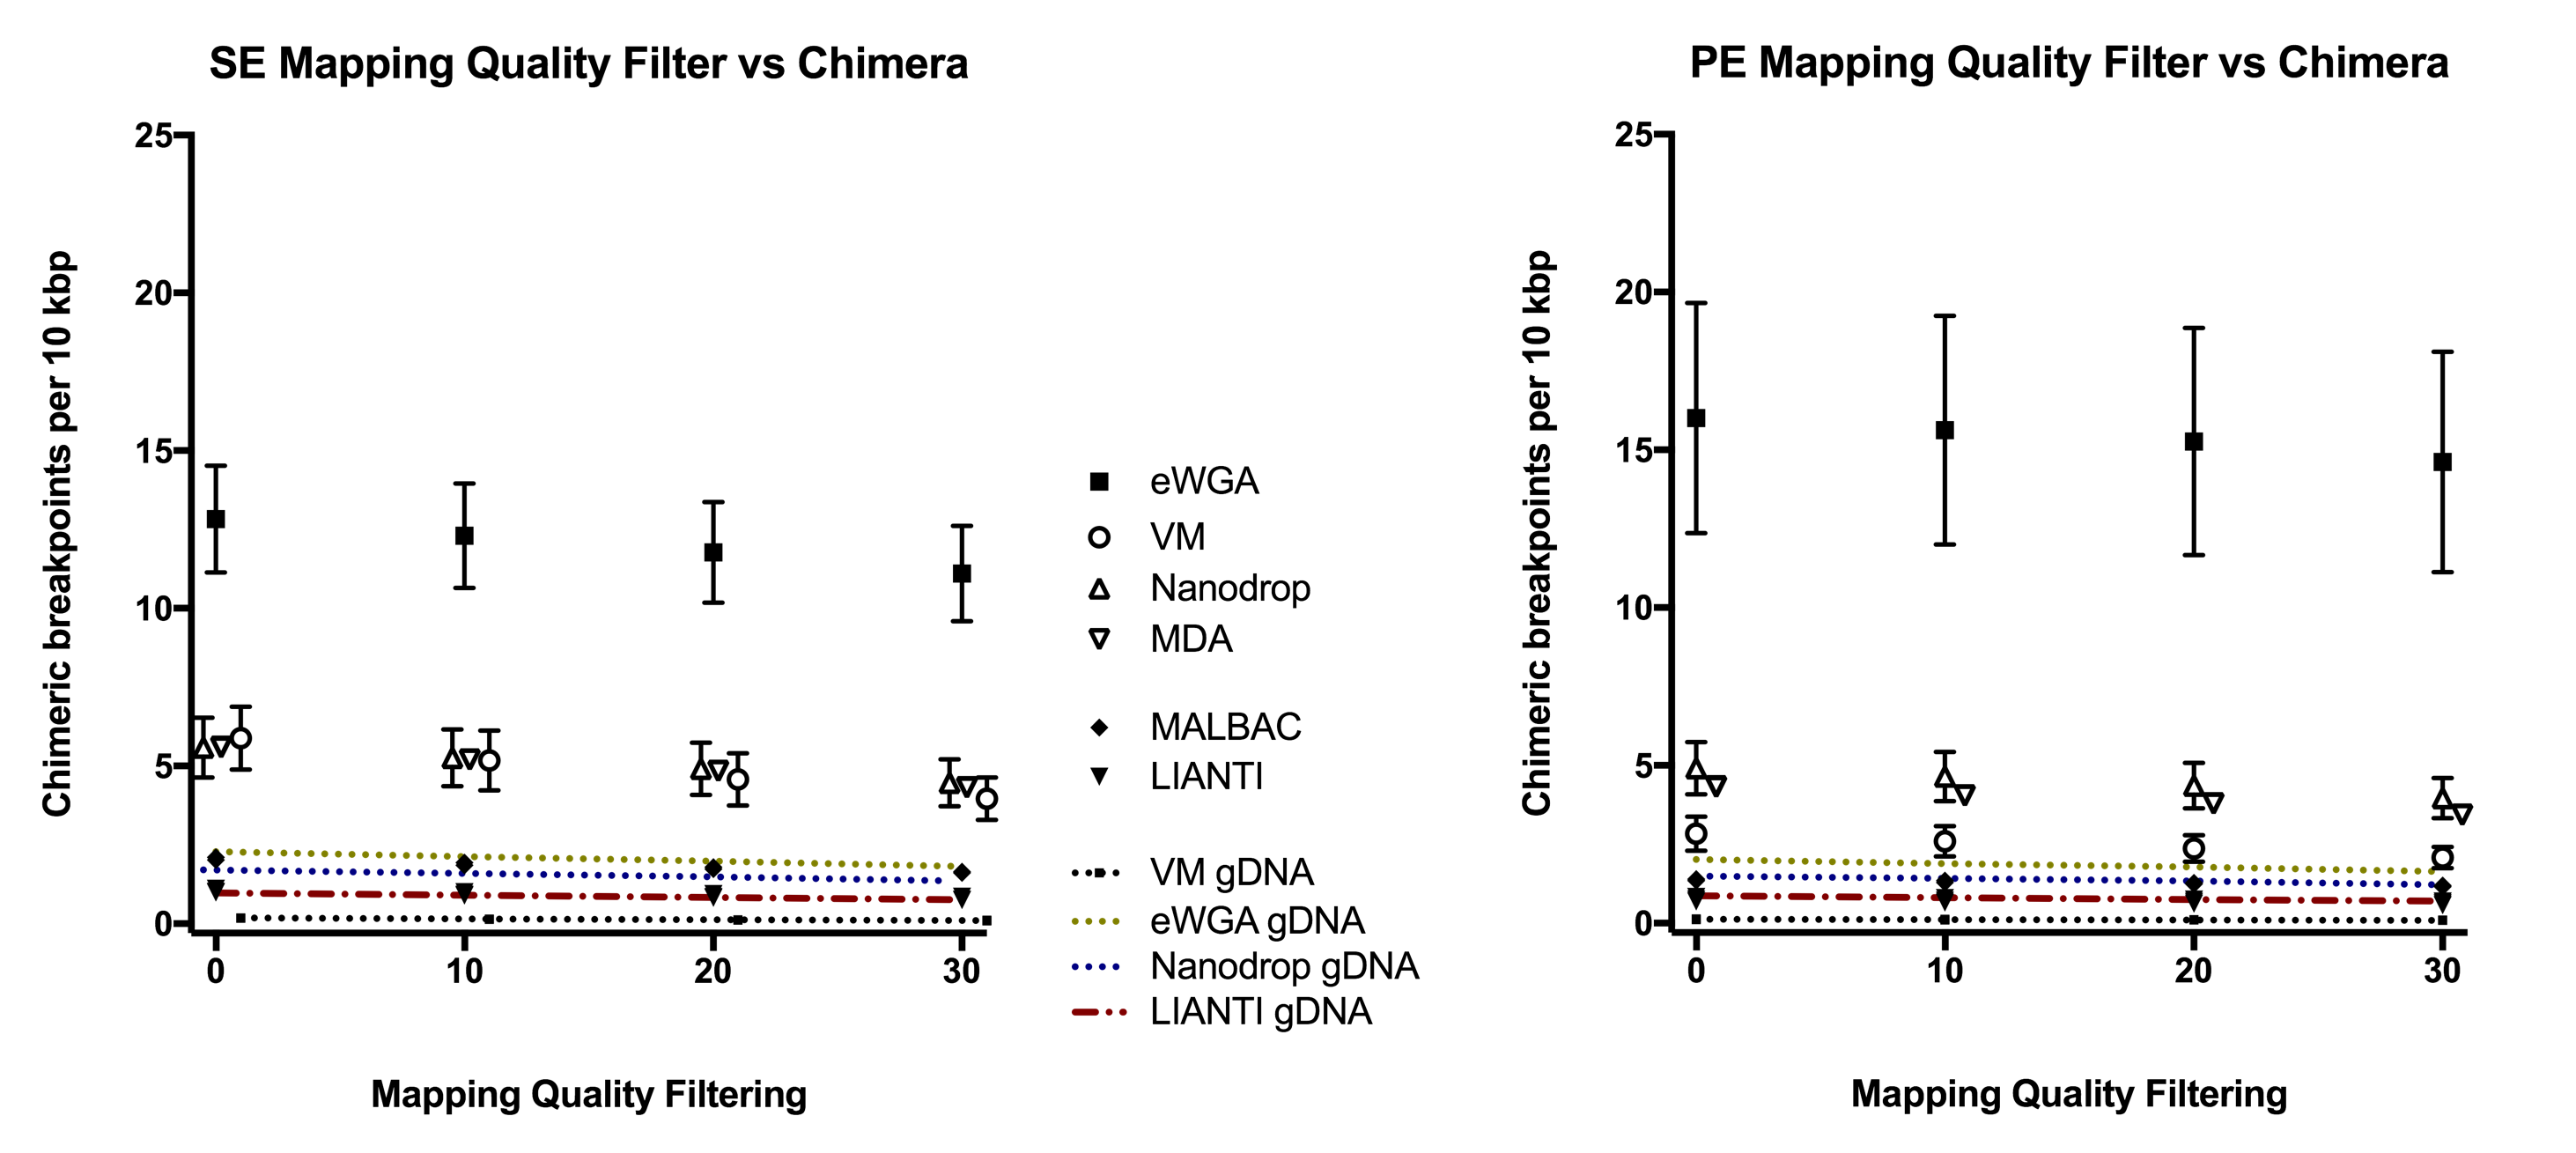
\includegraphics[keepaspectratio,width=\textwidth]{./figures/MappingQvsChimera}
\caption[The effect of mapping quality filtering on chimera detection.]{The effect of mapping quality filtering on chimera detection.}
\label{fig:chimeraMappingQAll}
\end{figure}

\begin{figure}
\centering
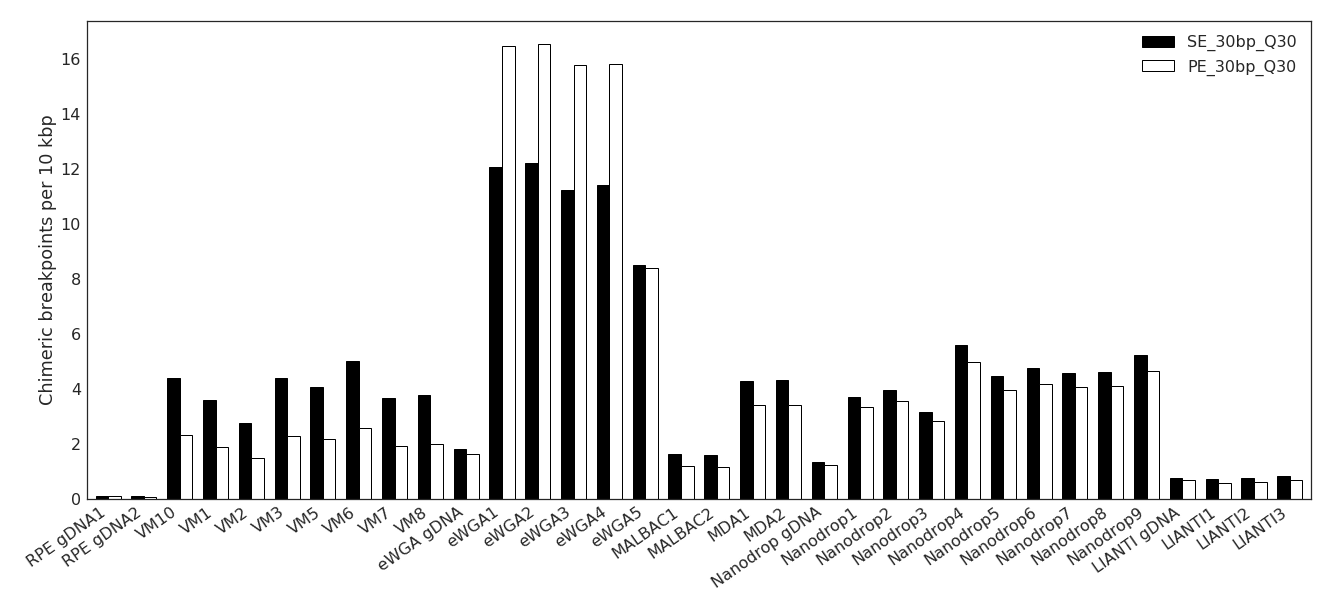
\includegraphics[keepaspectratio,width=1\textwidth]{./figures/20170517_ChimericBreakpoint10kbp_SEvsPE_Q30}
\caption[The effect of pair-ended and single-ended mapping on chimera detection]{The effect of pair-ended (PE) and single-ended (SE) mapping on chimera detection.}
\label{fig:chimeraPEvsSE}
\end{figure}

Most interestingly, we compared the effect of pair-ended and single-ended mapping on chimera detection (Fig. \ref{fig:chimeraPEvsSE}). For all datasets except eWGA, single-ended mapping analysis overestimates chimera rate compared to pair-ended mapping with the same downsampled reads. With pair-ended mapping, read pairs mapped within the range of insert size with the correct orientation is chosen as the primary mapping results. With the single-ended mapping, reads that mapped to multiple locations equally well were randomly chosen for the final output, thus, causing an overestimation of chimeric read out of total mapped reads. For eWGA, there is a 50\% increase of chimera frequency by pair-ended mapping compared to single-ended mapping. This increase can be explained by the especially high content of inverted chimera that can be easily detected in the pair-end mode. In the single-end mode, a potential inverted chimera might be able to map to a reverse-complementary location with the same mapping quality, and thus, the single-end mode underestimate the chimera rate. We are uncertain about why VM samples are affected the most by PE vs SE mapping ($\sim$ 50\% change). Possible explanations include the differences between cell lines, library preparation procedures and the nature of DNA amplification in hydrogel. Further experiments will be needed to validate the cause. 

\begin{figure}
\centering
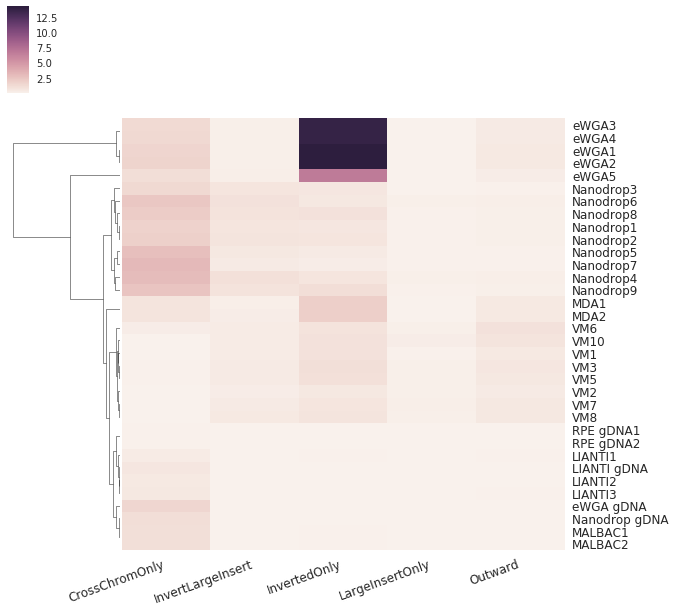
\includegraphics[keepaspectratio,width=1\textwidth]{./figures/20170822_BreakpointPer10kbp_Clustermap_QFiltered}
\caption[Hierarchical clustering of chimera breakpoints per 10 kbp.]{Hierarchical clustering of chimera breakpoints per 10 kbp for each single cells and genomic DNA controls.\textit{Virtual Microfluidics} samples are closely clustered with genomic DNA controls, indicating low levels of chimera generated by hydrogel MDA}
\label{fig:chimeraCluster}
\end{figure}

Furthermore, by hierarchically clustering the datasets based on their chimera signatures (Fig. \ref{fig:chimeraCluster}), we see the close similarities between \textit{virtual microfluidics} samples and the LIANTI single cells in terms of chimera rate, while most of the nanodrop datasets are closely clustered with traditional MDA reactions. MALBAC samples are clustered with gDNA controls with PCR-enriched chimera baseline. LIANTI samples are closely clustered with PCR-free gDNA controls that represent chimera-free negative control, which indicates the \textit{in vitro} transcription amplification could generate minimal chimera. 

% \begin{figure}
% \centering
% 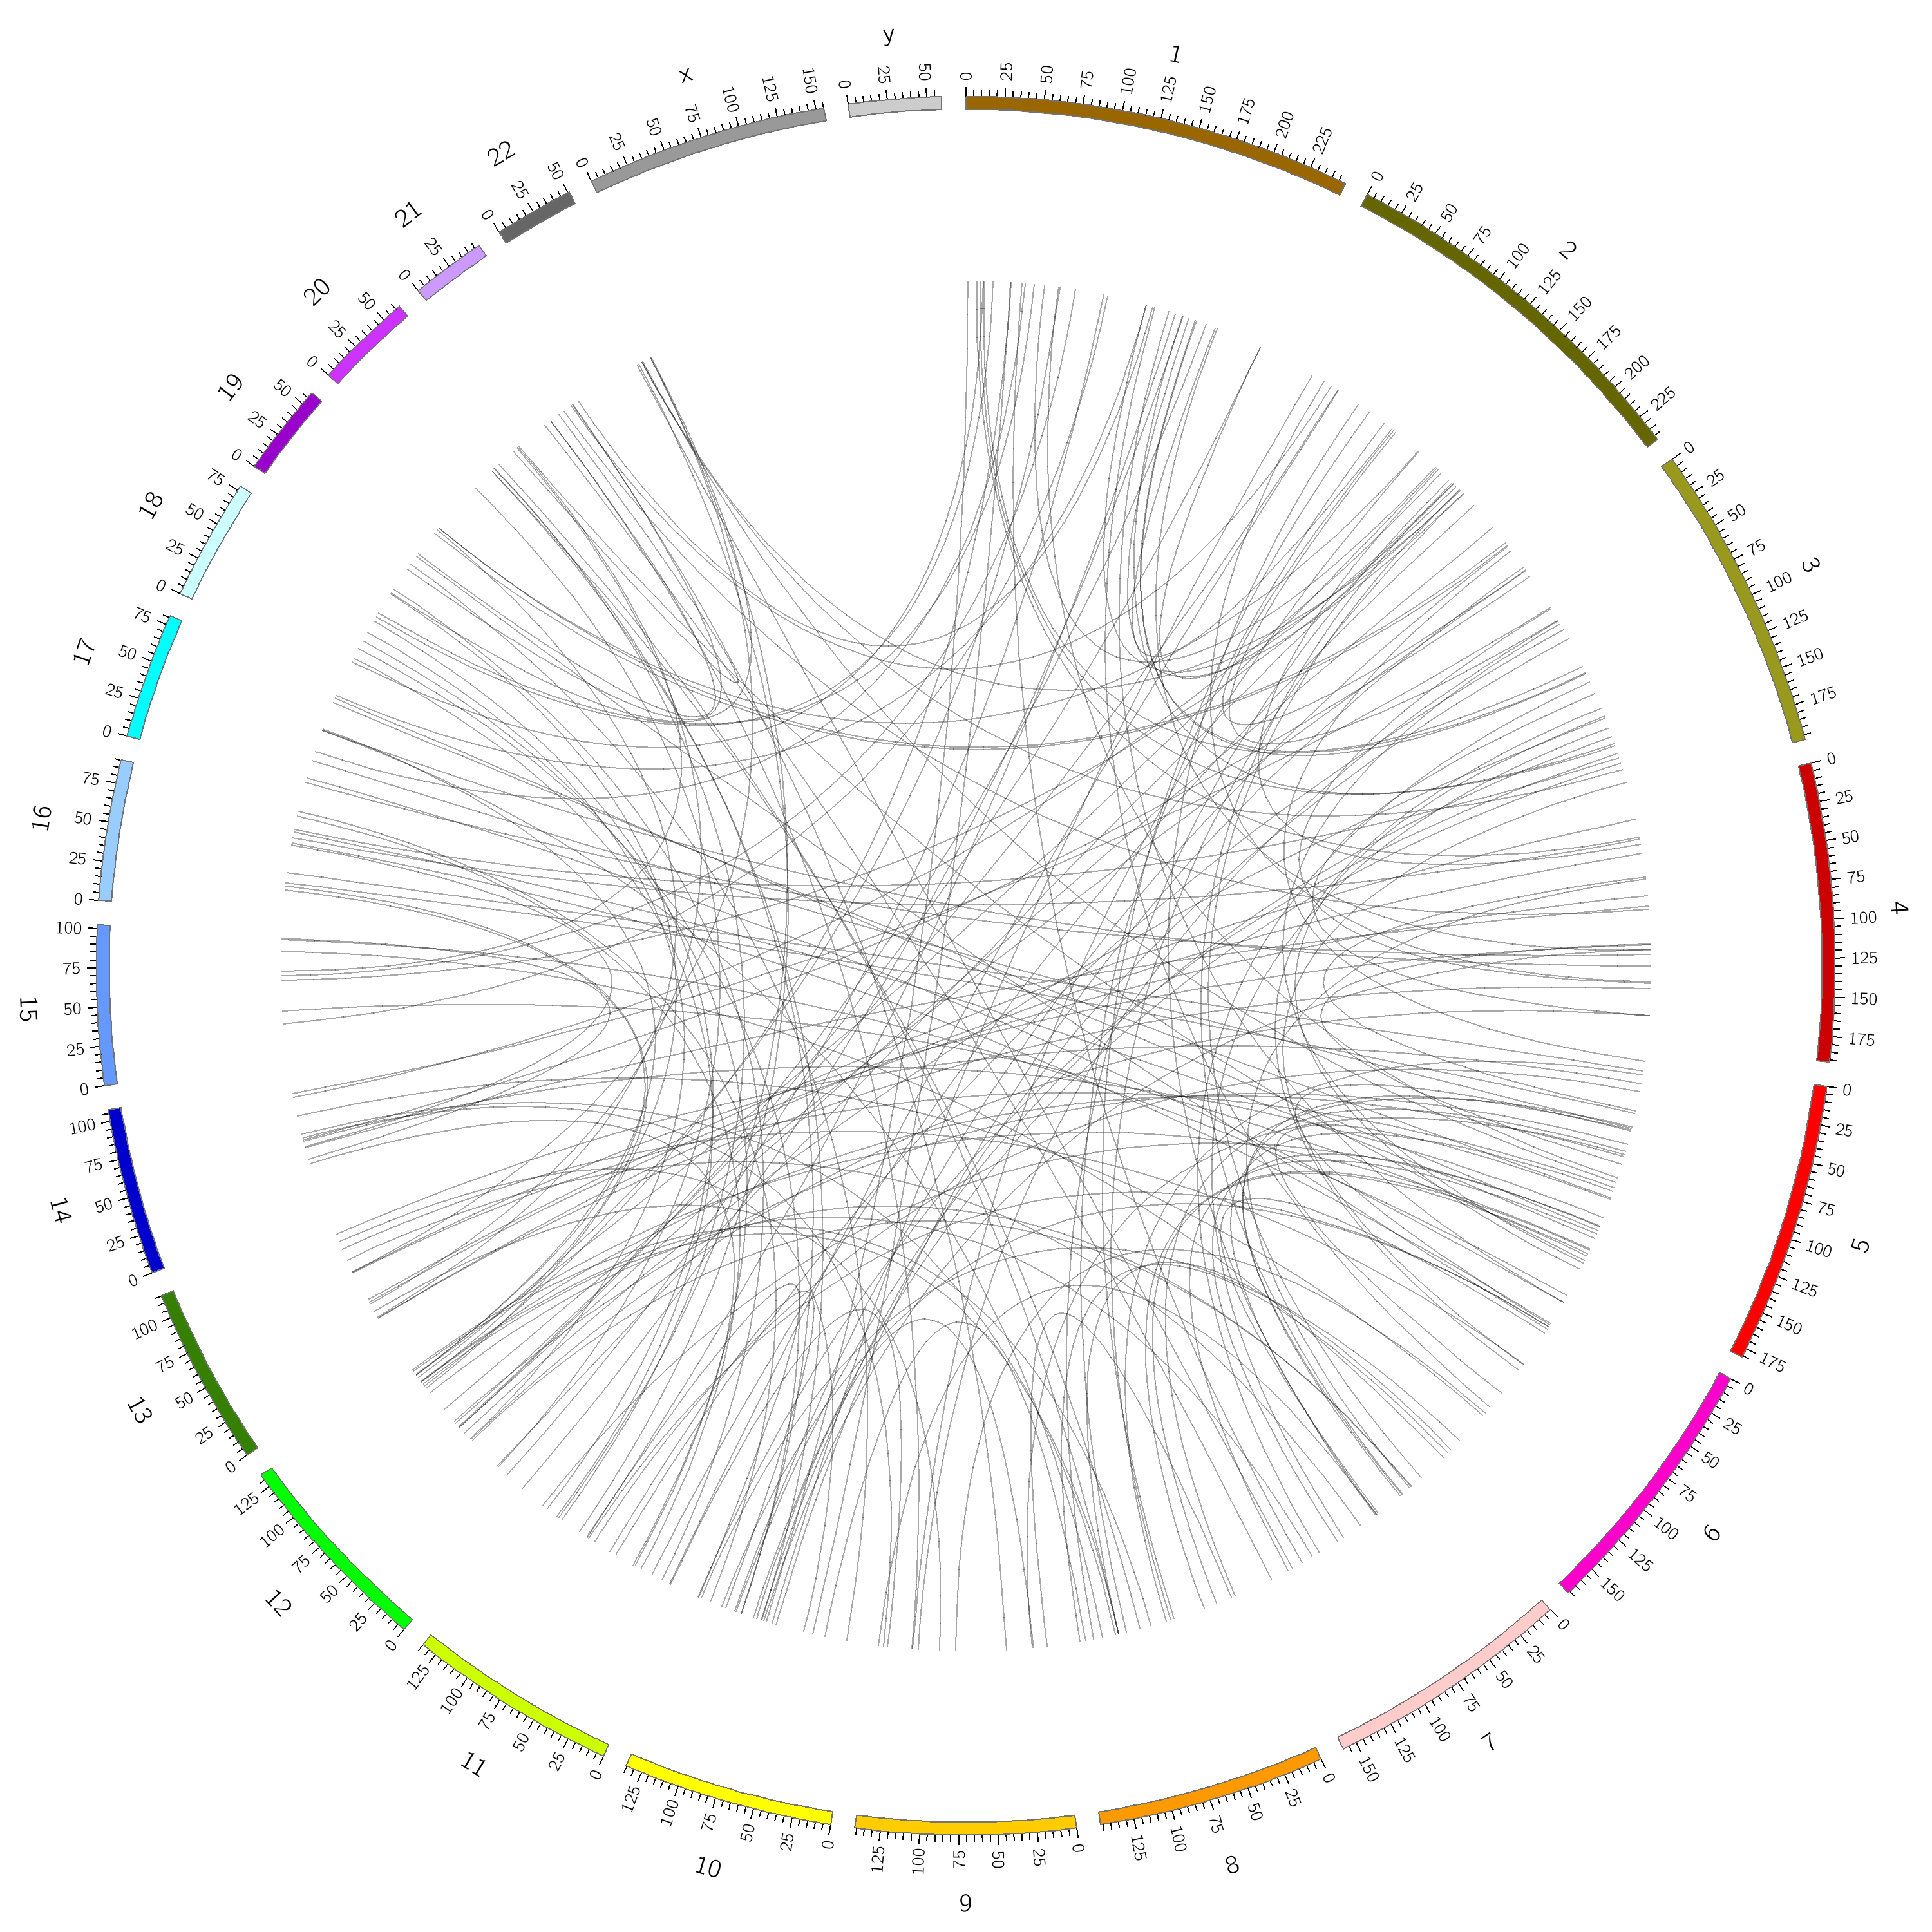
\includegraphics[keepaspectratio,width=1\textwidth]{./figures/LX0gDNAcircos}
% \caption[Cross-chromosome chimera map for RPE genomic DNA]{Cross-chromosome chimera map for RPE genomic DNA. Cross-chromosome chimera pairs are connected, shown as the black lines.}
% \label{fig:LX0gDNAcircos}
% \end{figure}

\begin{figure}
\begin{tabular}{cc}
VM gDNA (PCR free) & VM 1 \\
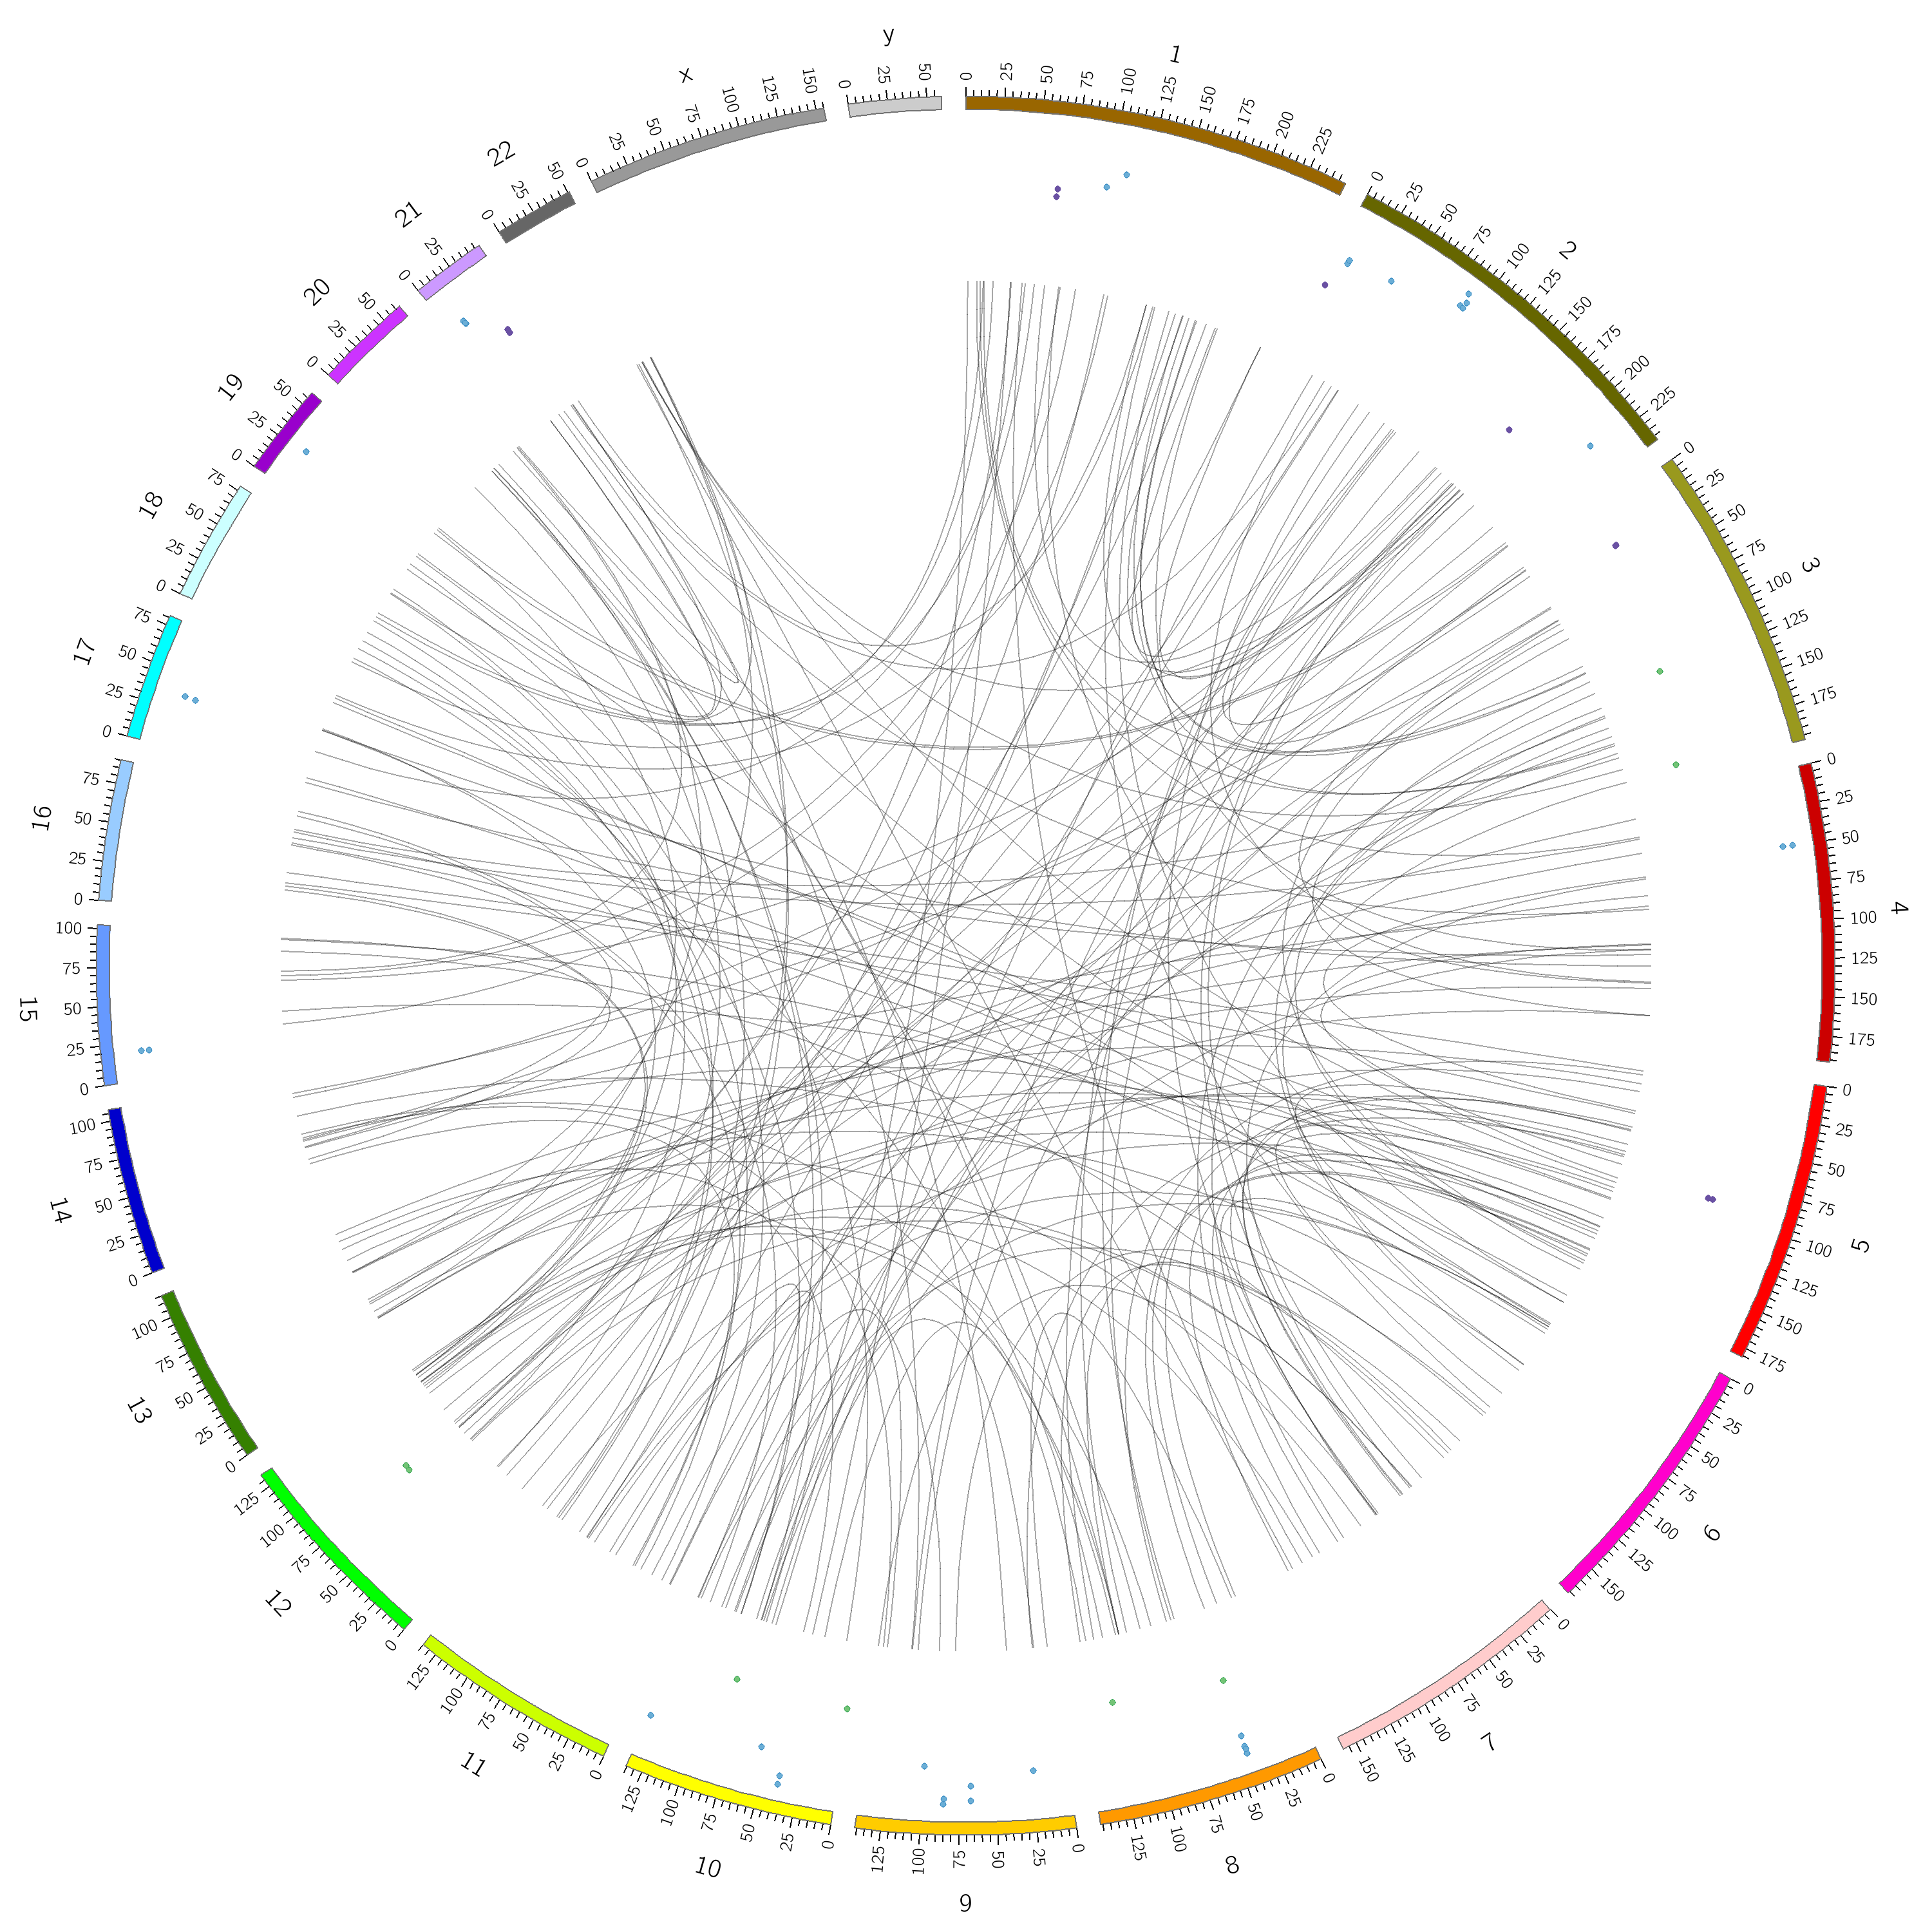
\includegraphics[keepaspectratio,width=0.5\textwidth]{./figures/circos/LX0gDNA_0529} & 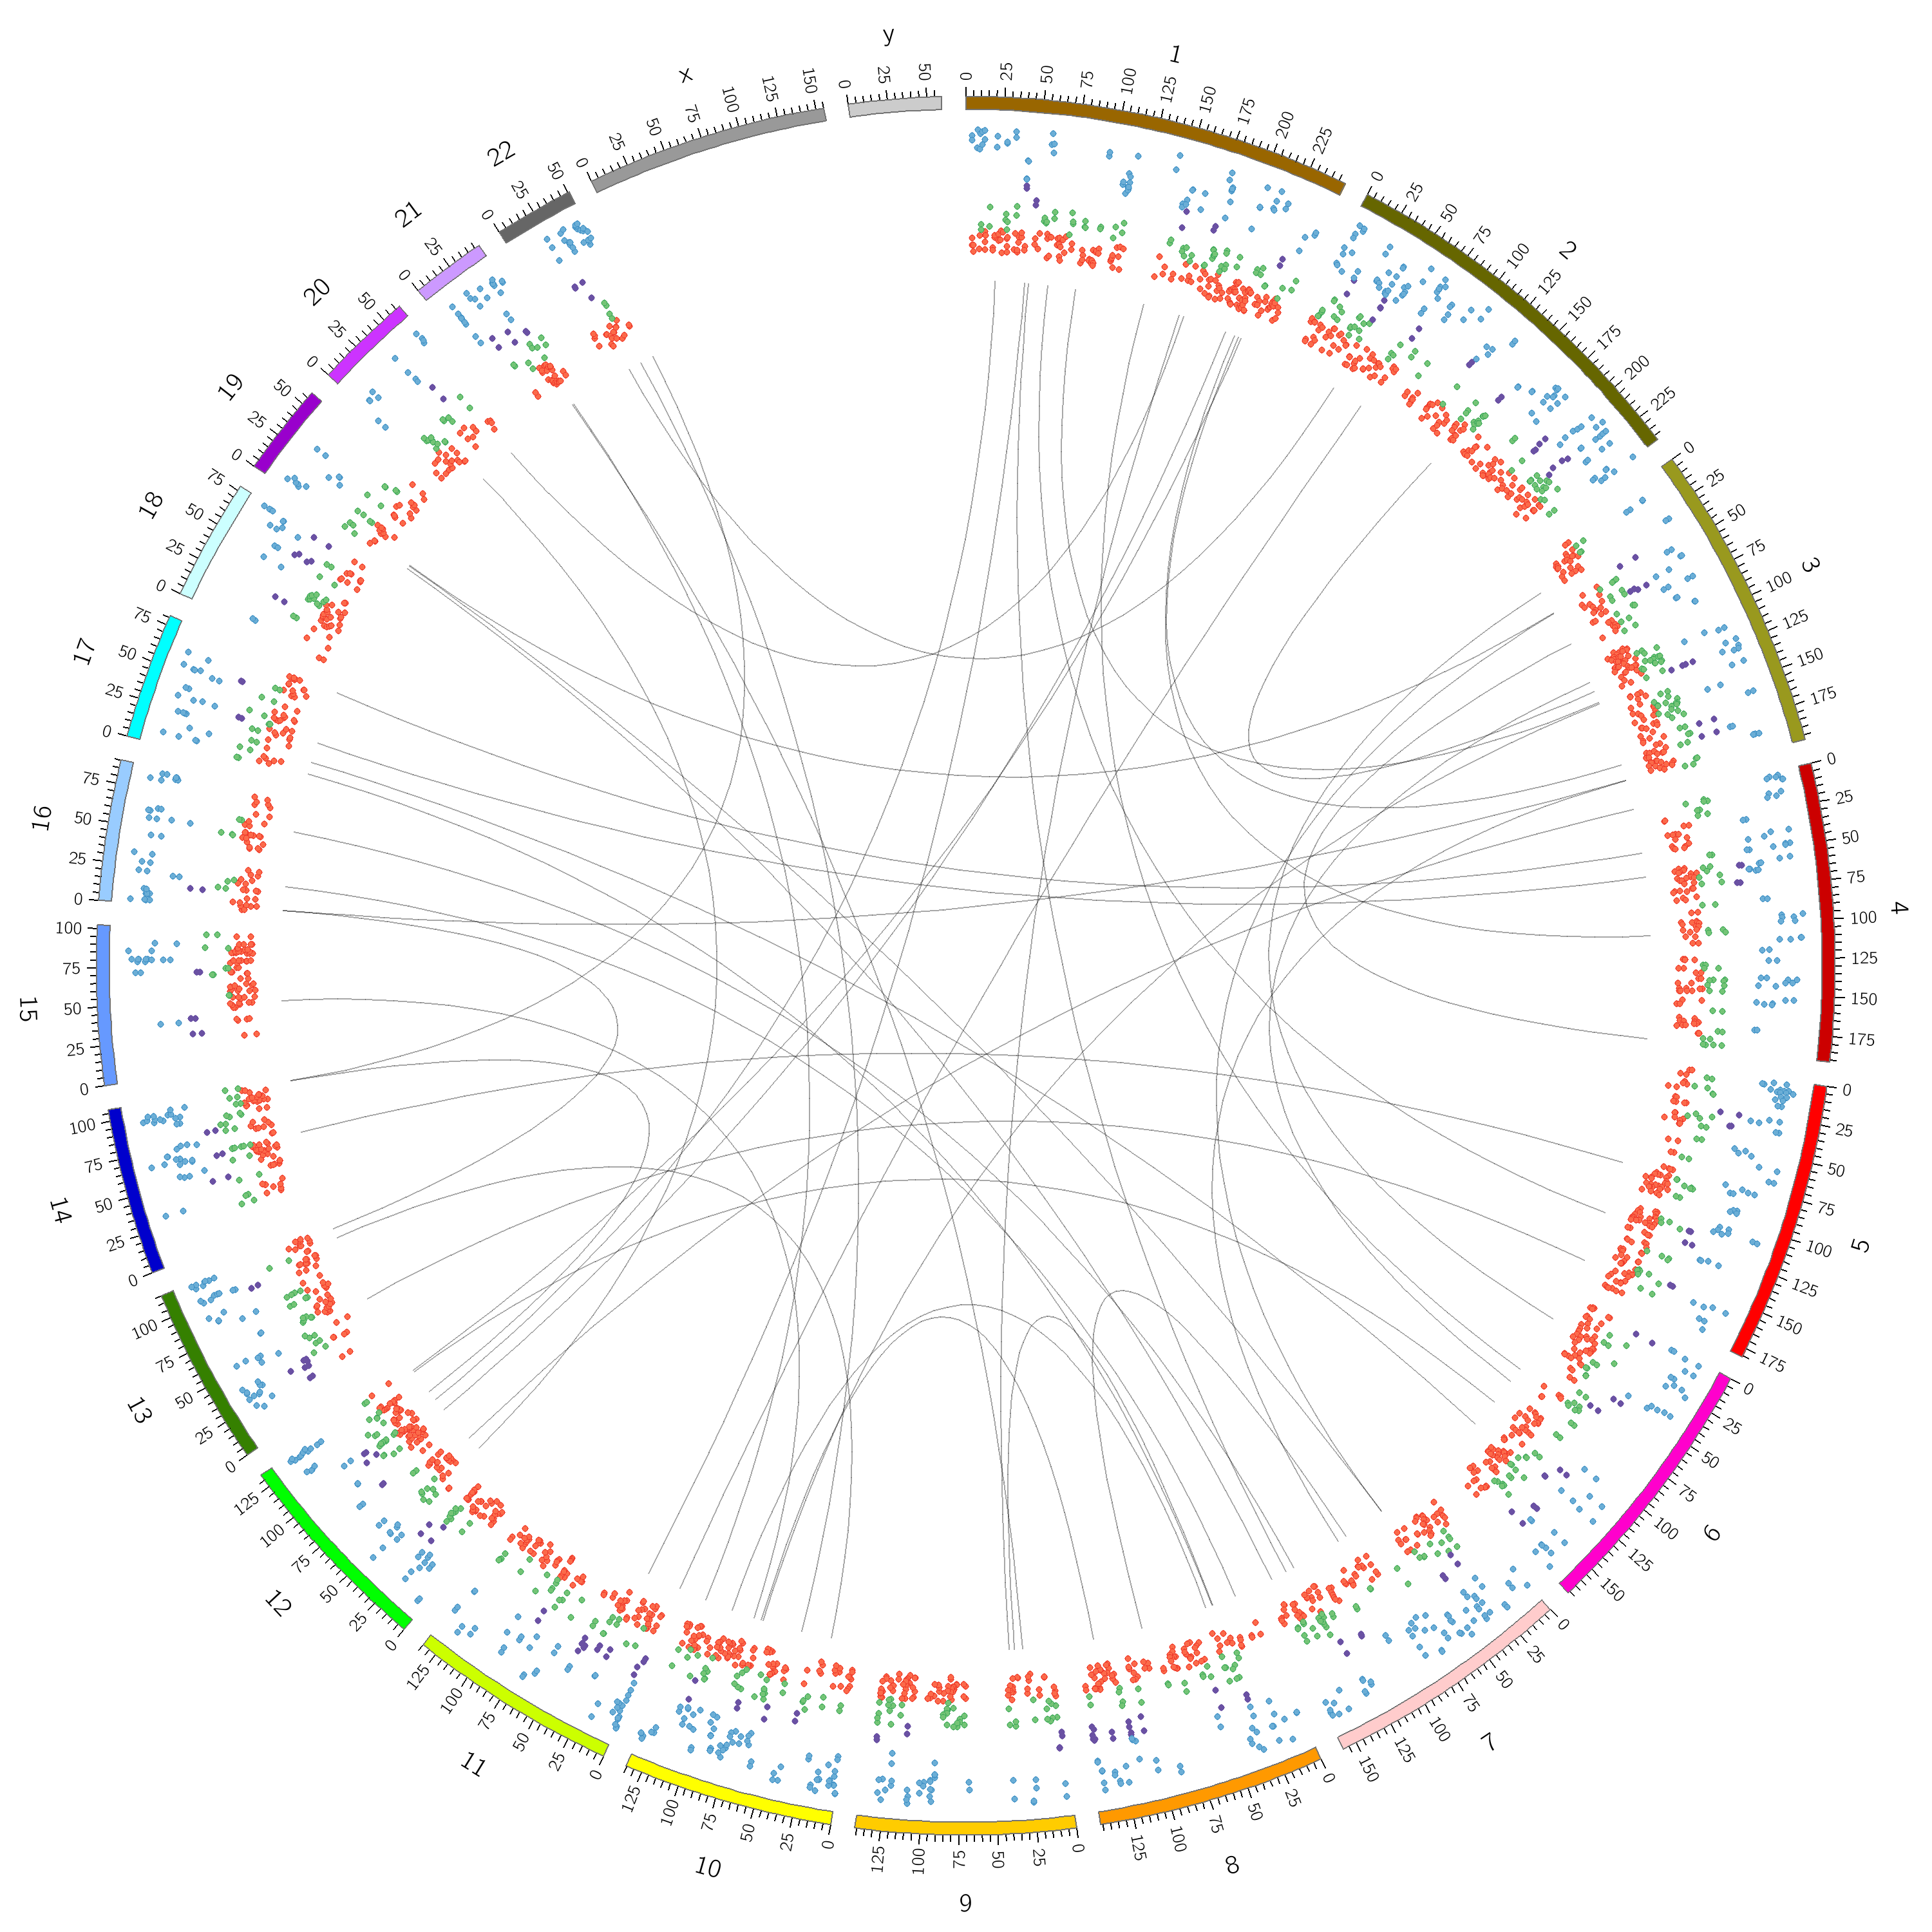
\includegraphics[keepaspectratio,width=0.5\textwidth]{./figures/circos/LX1_0529} \\
eWGA gDNA & eWGA 1 \\
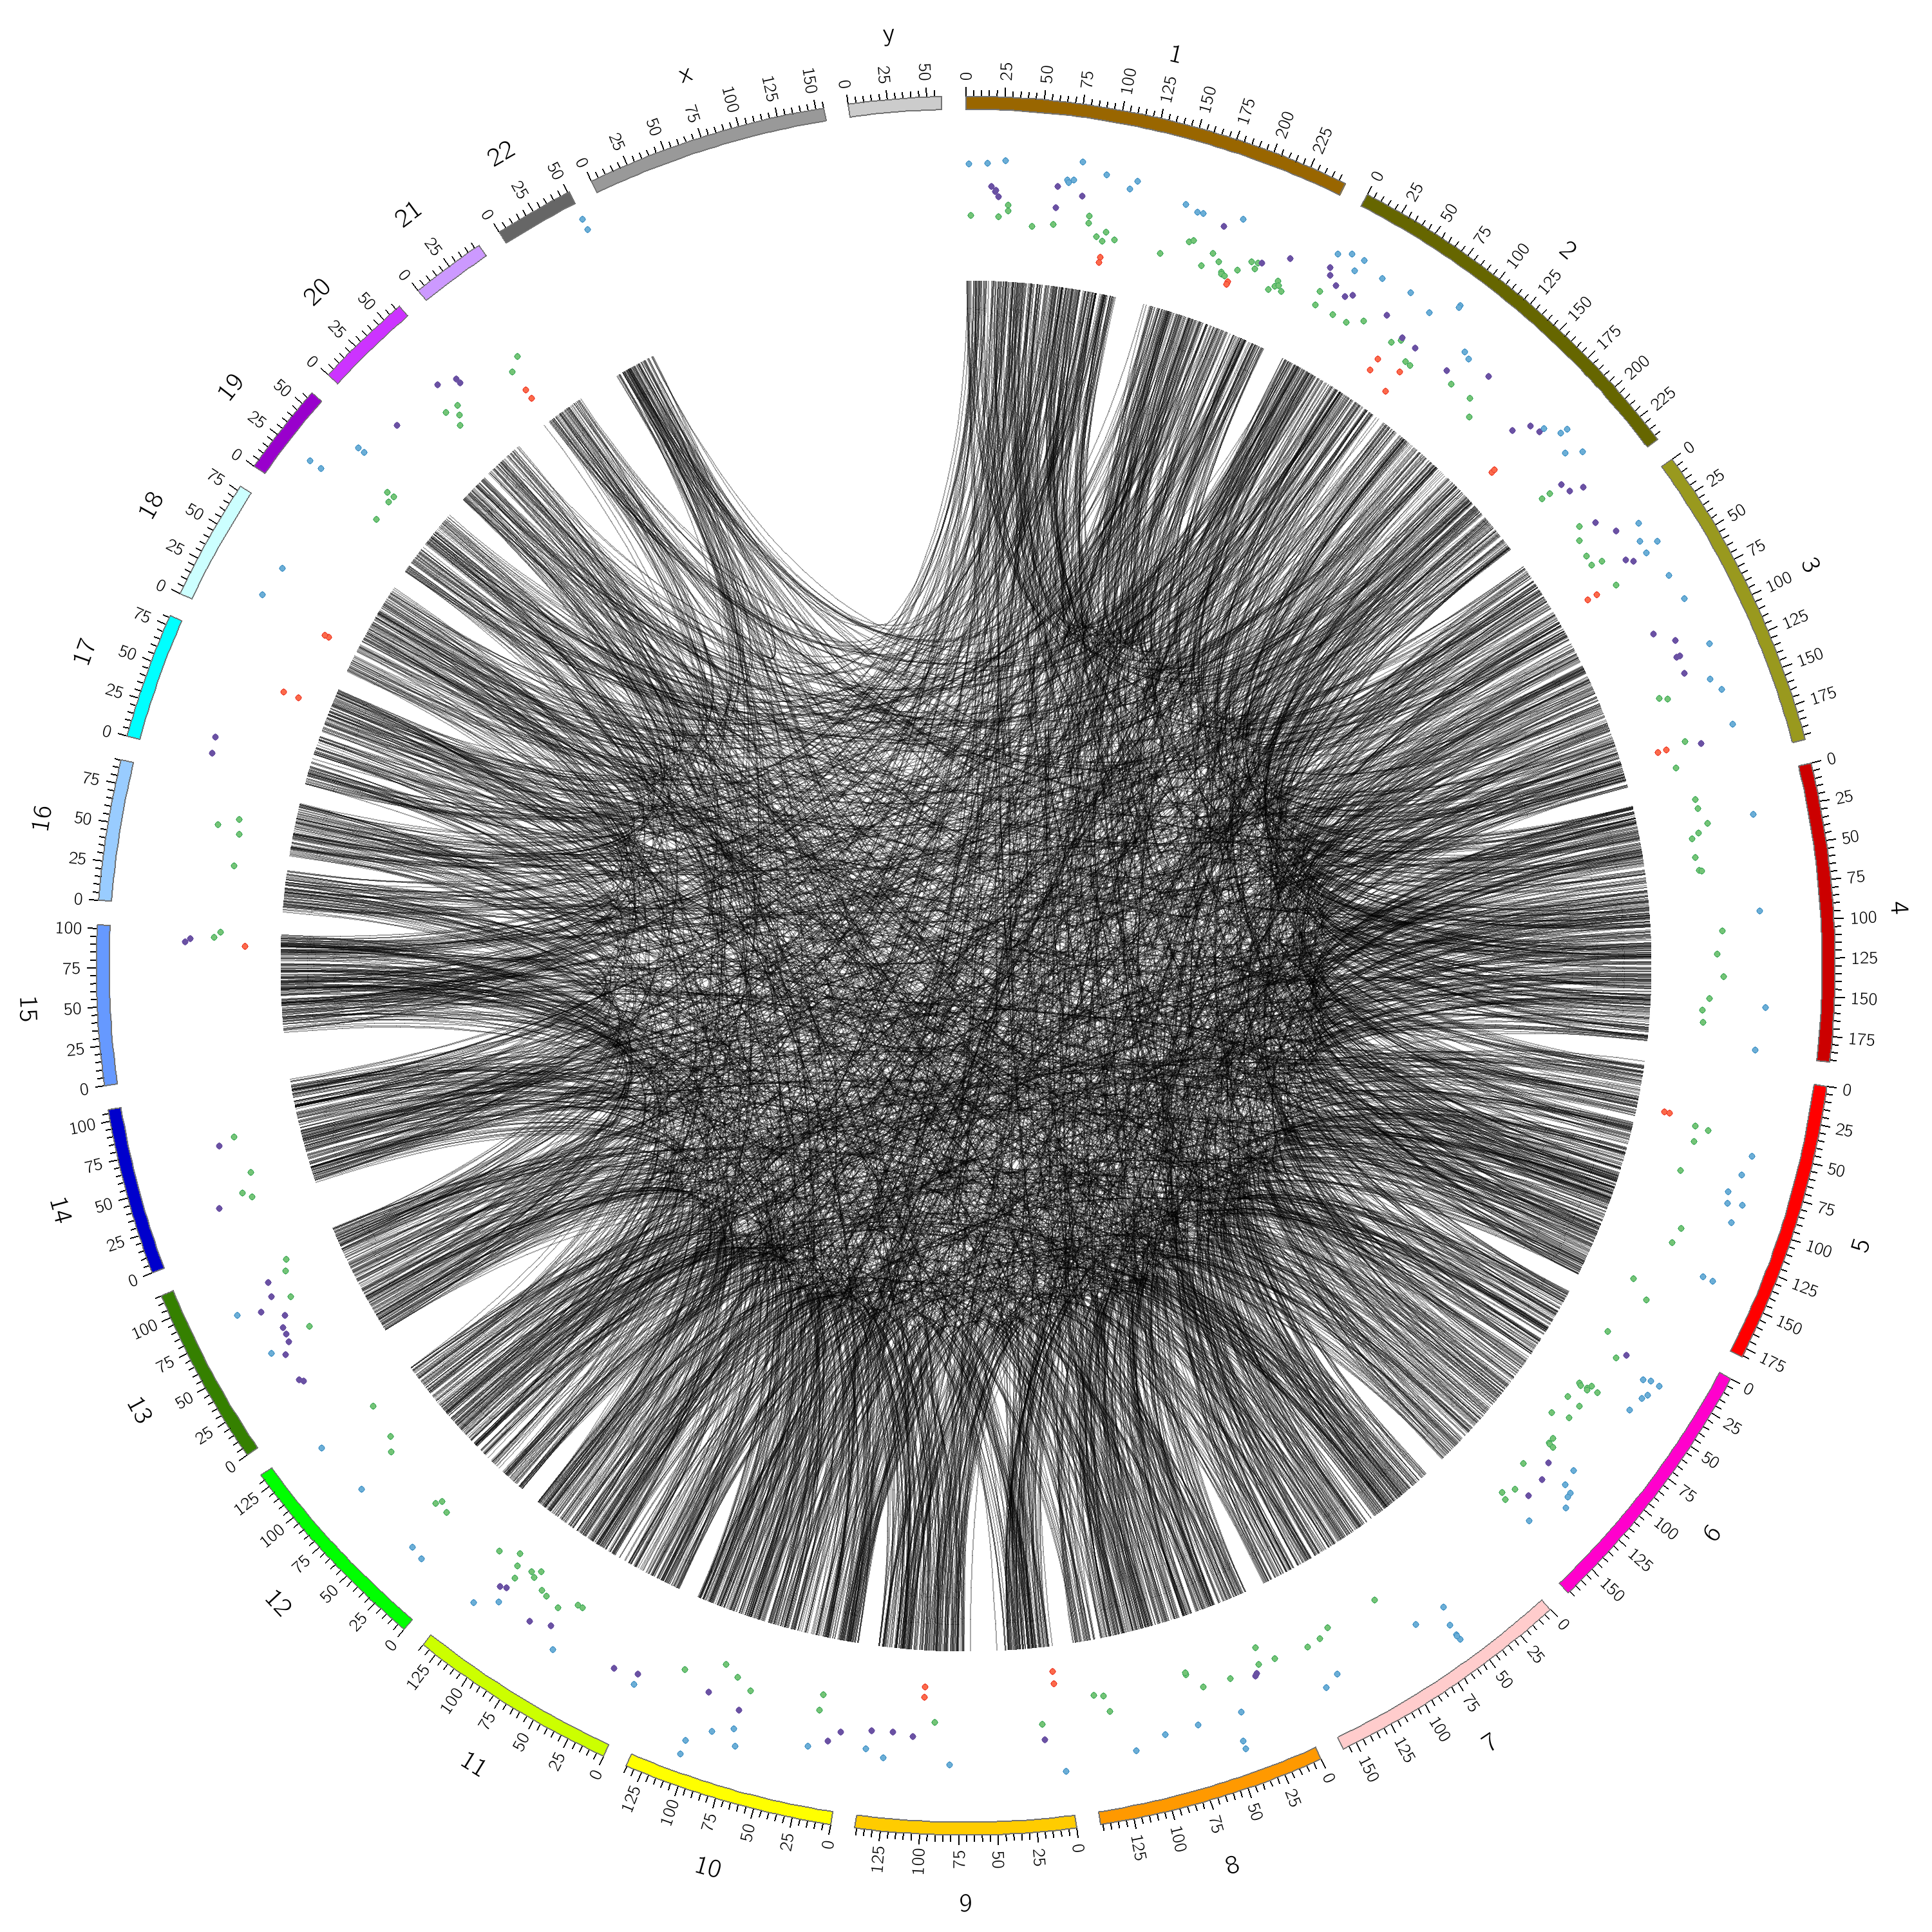
\includegraphics[keepaspectratio,width=0.5\textwidth]{./figures/circos/SRR1777284gDNA_0529} & 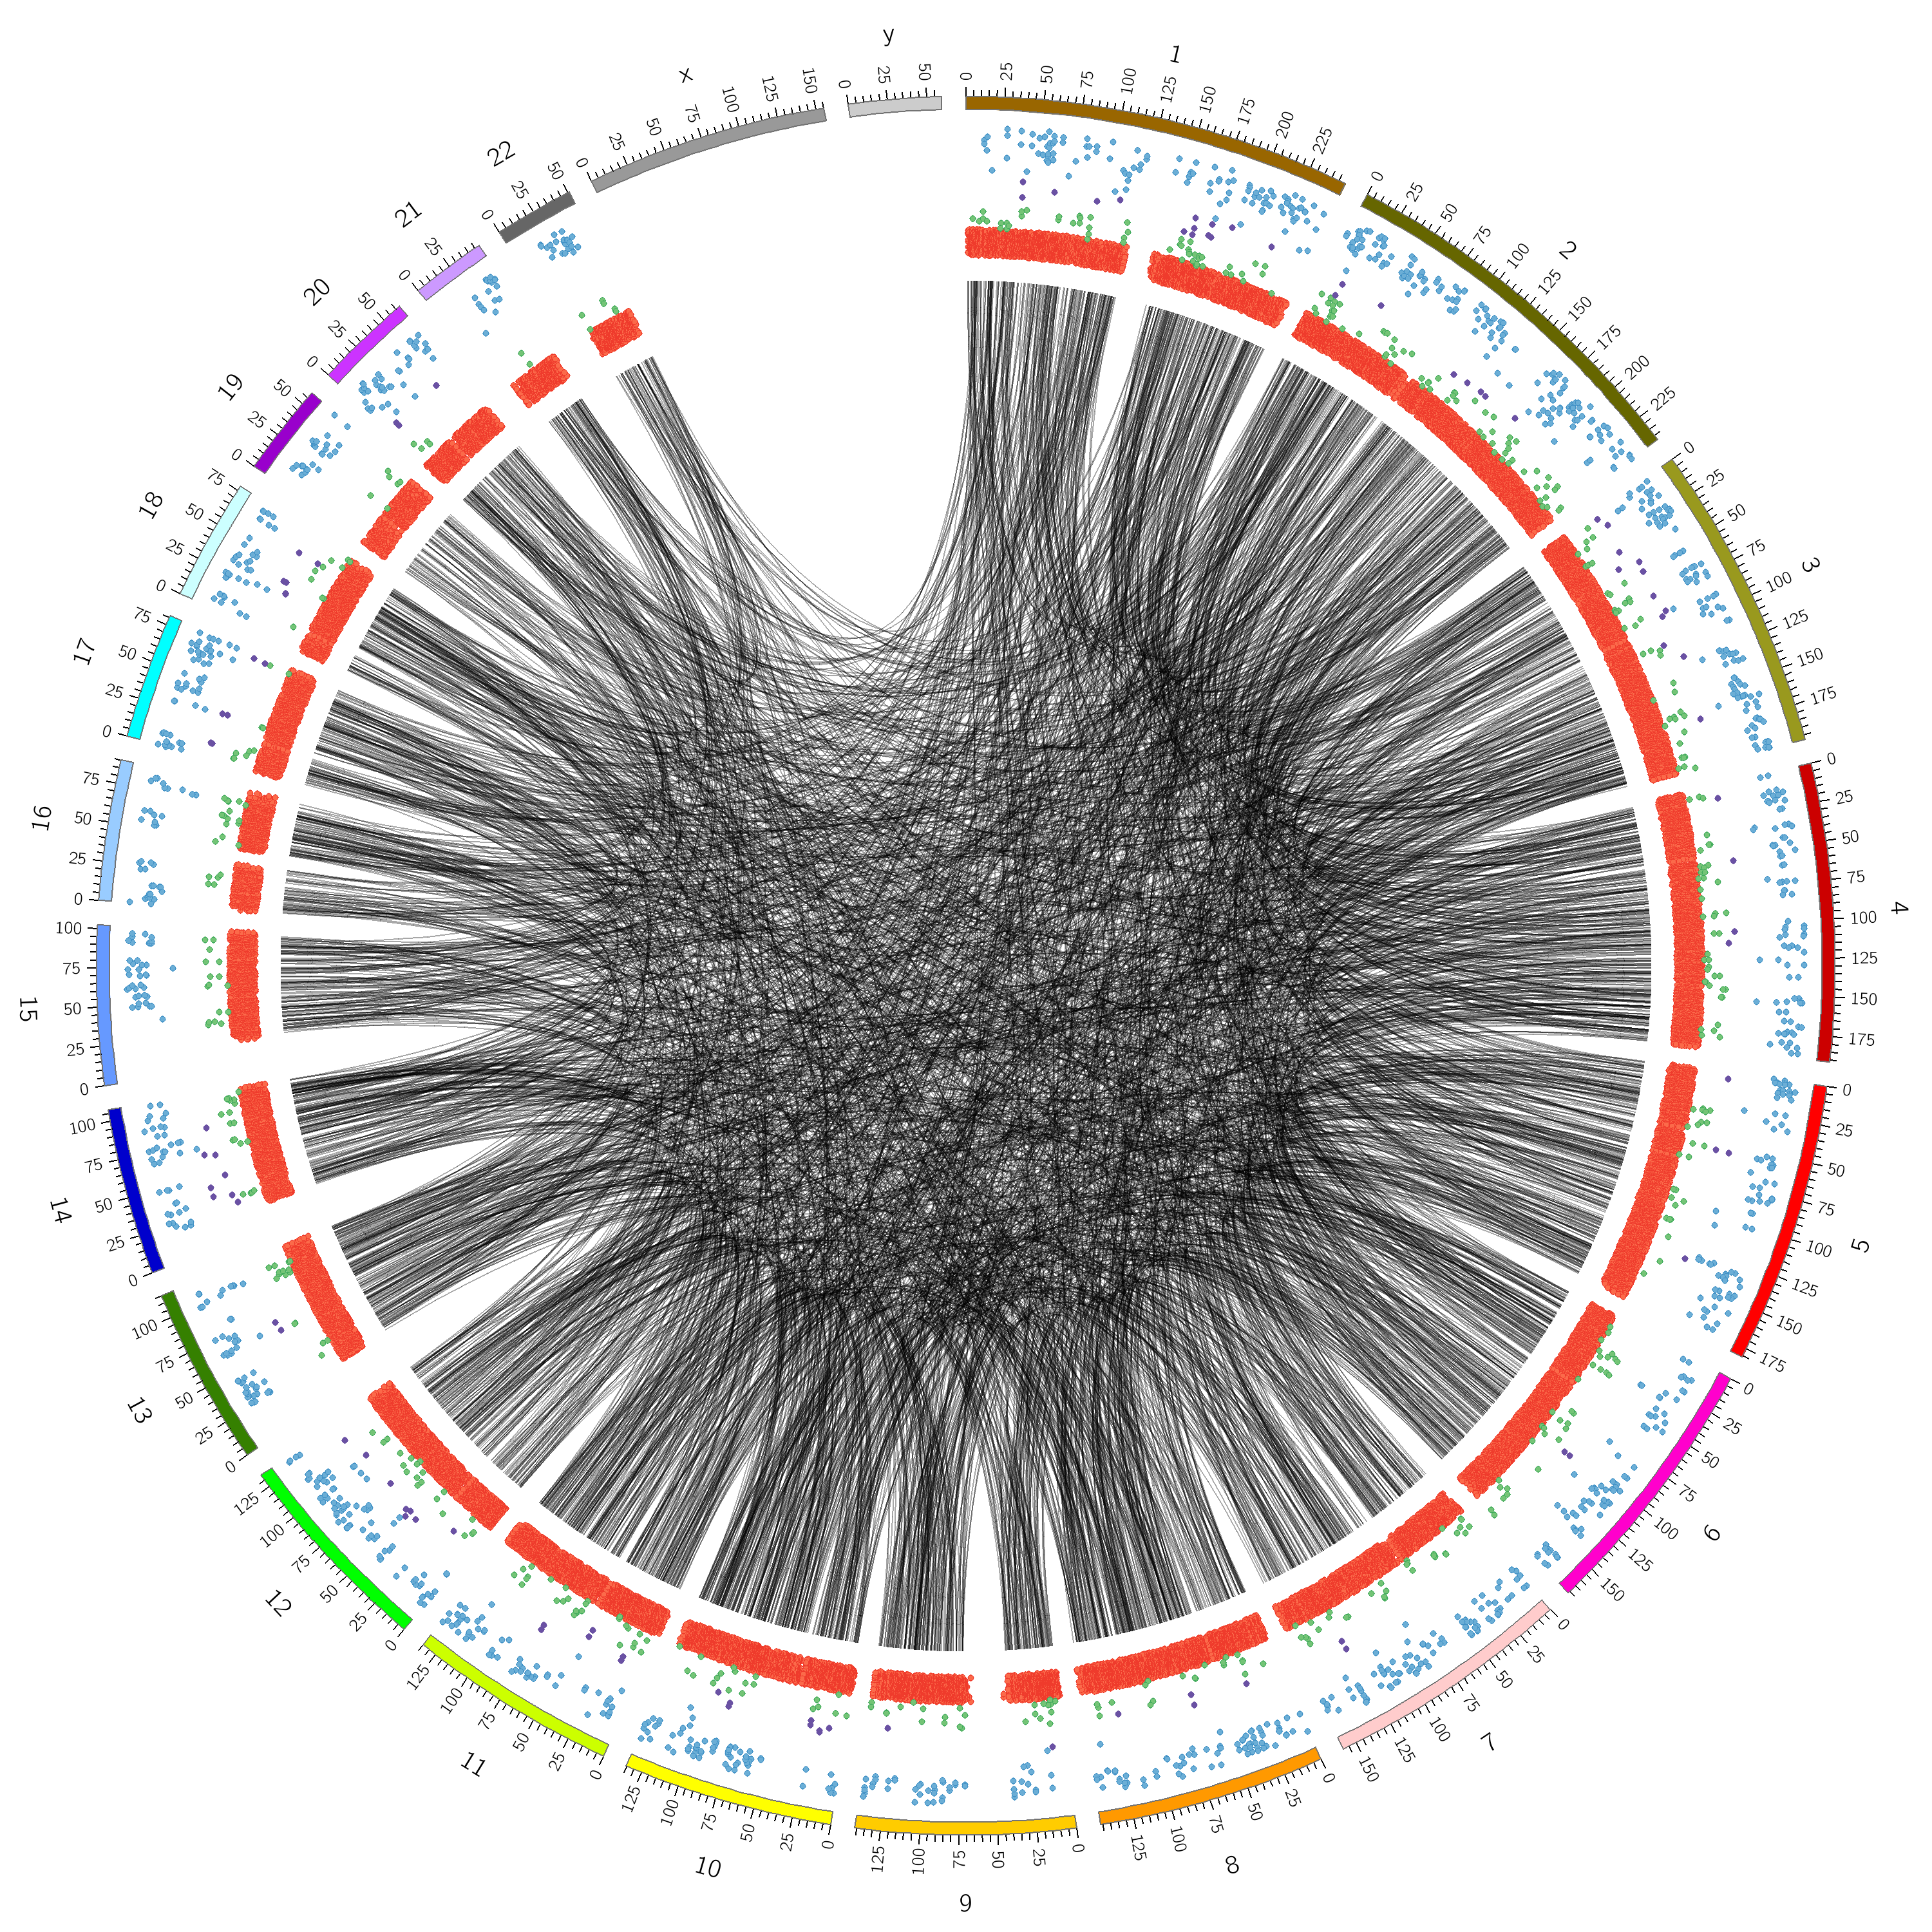
\includegraphics[keepaspectratio,width=0.5\textwidth]{./figures/circos/SRR1777287_0529} \\
\end{tabular}
\caption[Chimera breakpoints shown in Circos plots (part 1)]{Chimera breakpoints shown in Circos plots for bulk genomic DNA and single-cell samples (part 1). Cross-chromosome chimera pairs are connected, shown as black lines in the center. Inverted chimera breakpoints are represented as red dots. Inverted \& large-insert chimera breakpoints are green dots. Large-insert chimera breakpoints are purple dots. Outward chimera breakpoints are blue dots.}
\label{fig:LX0gDNAcircos}
\end{figure}

\begin{figure}
\begin{tabular}{cc}
Nanodrop gDNA & Nanodrop 1 \\
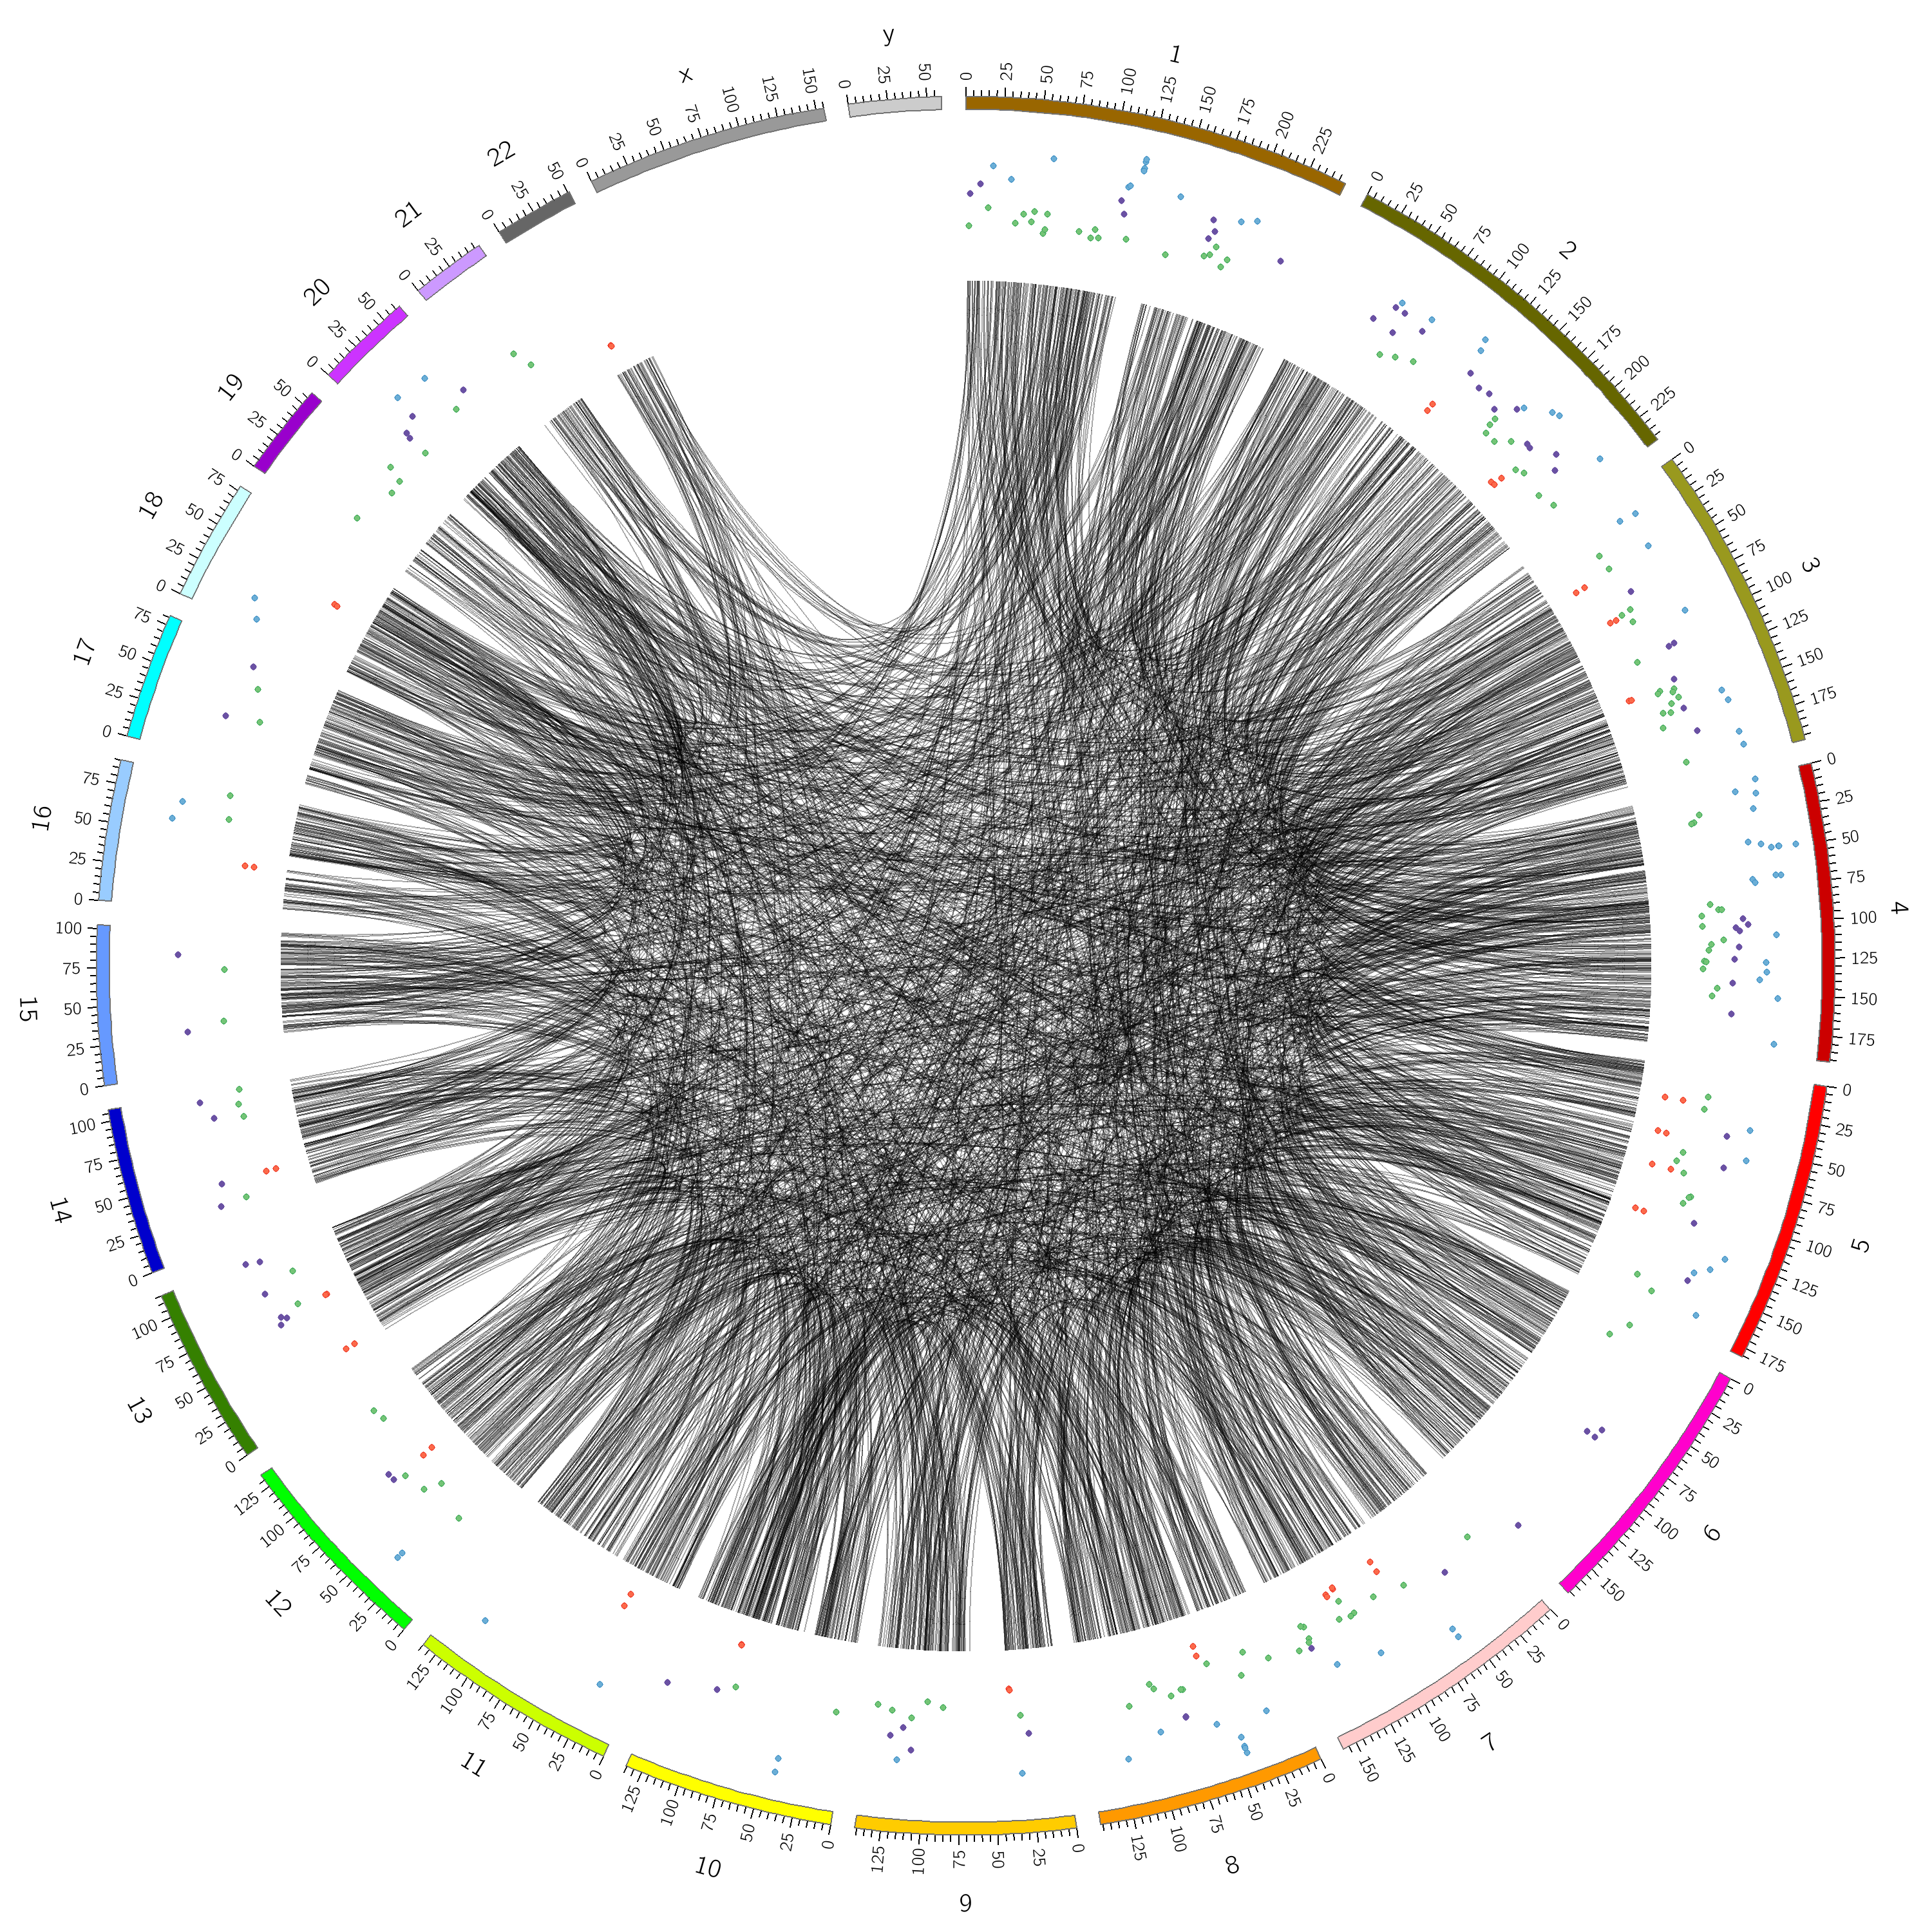
\includegraphics[keepaspectratio,width=0.5\textwidth]{./figures/circos/SRR3749000gDNA_0529} & 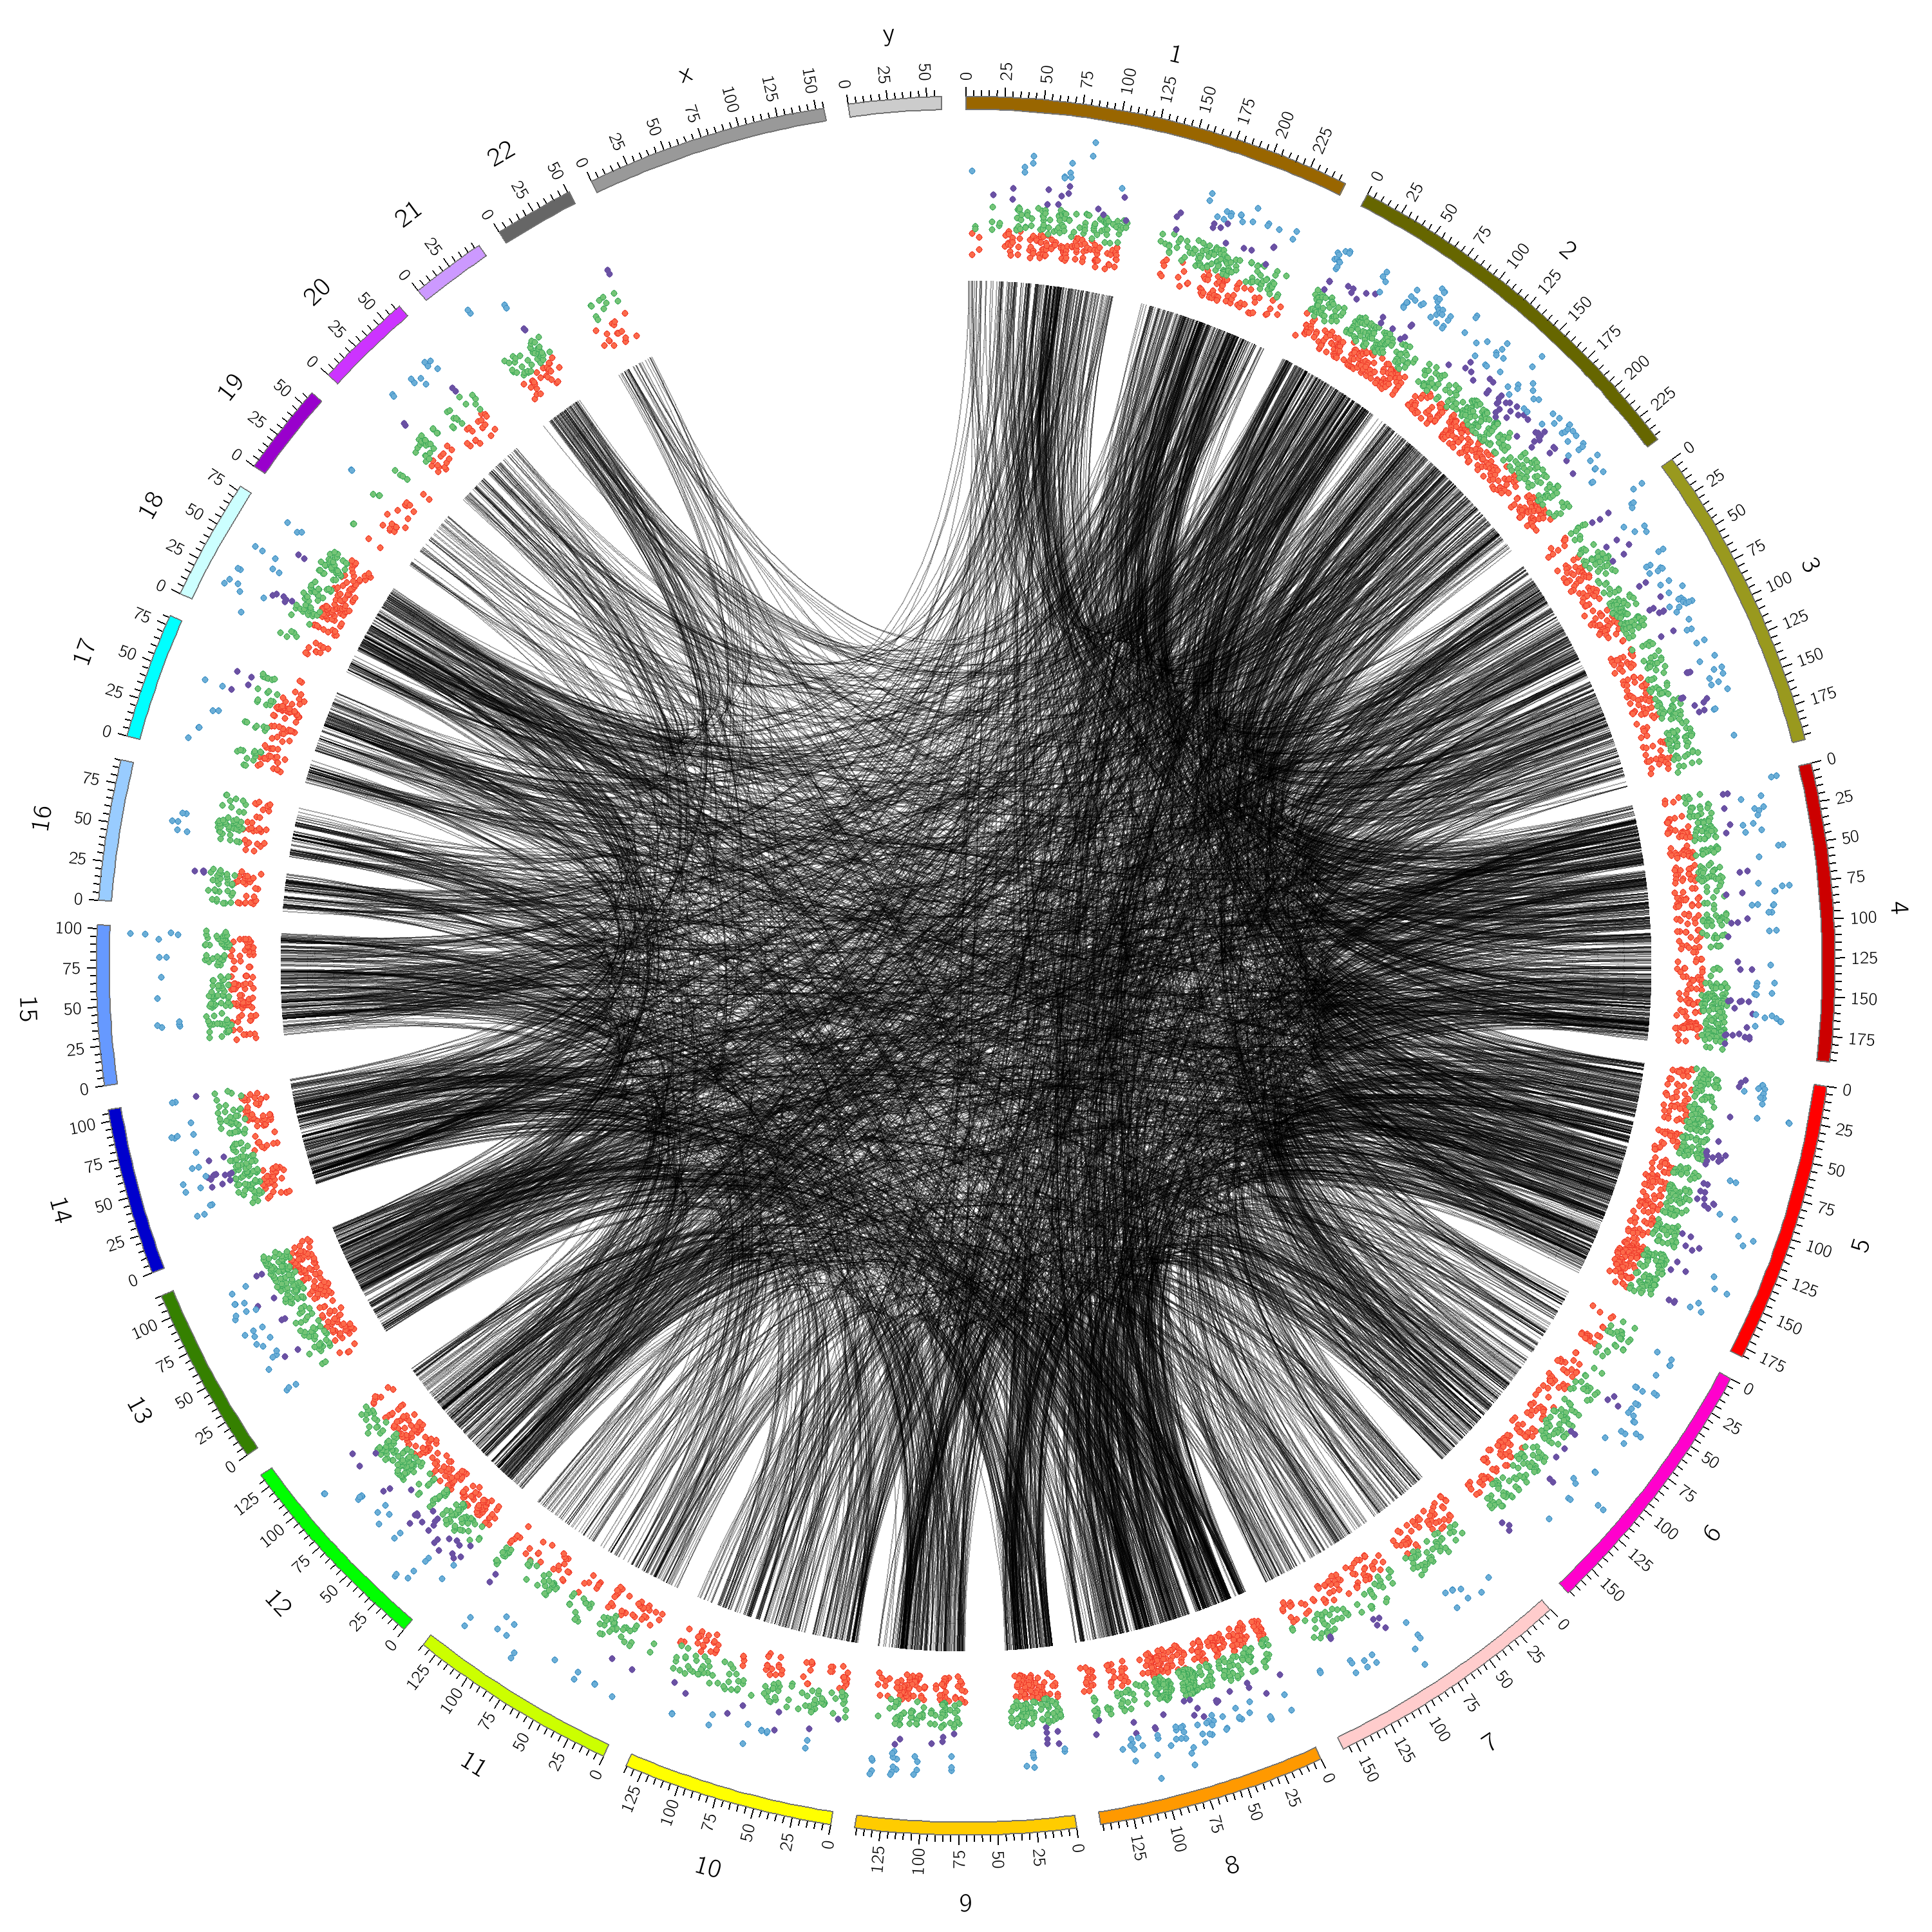
\includegraphics[keepaspectratio,width=0.5\textwidth]{./figures/circos/SRR3749174_0529} \\
LIANTI gDNA & LIANTI 1 \\
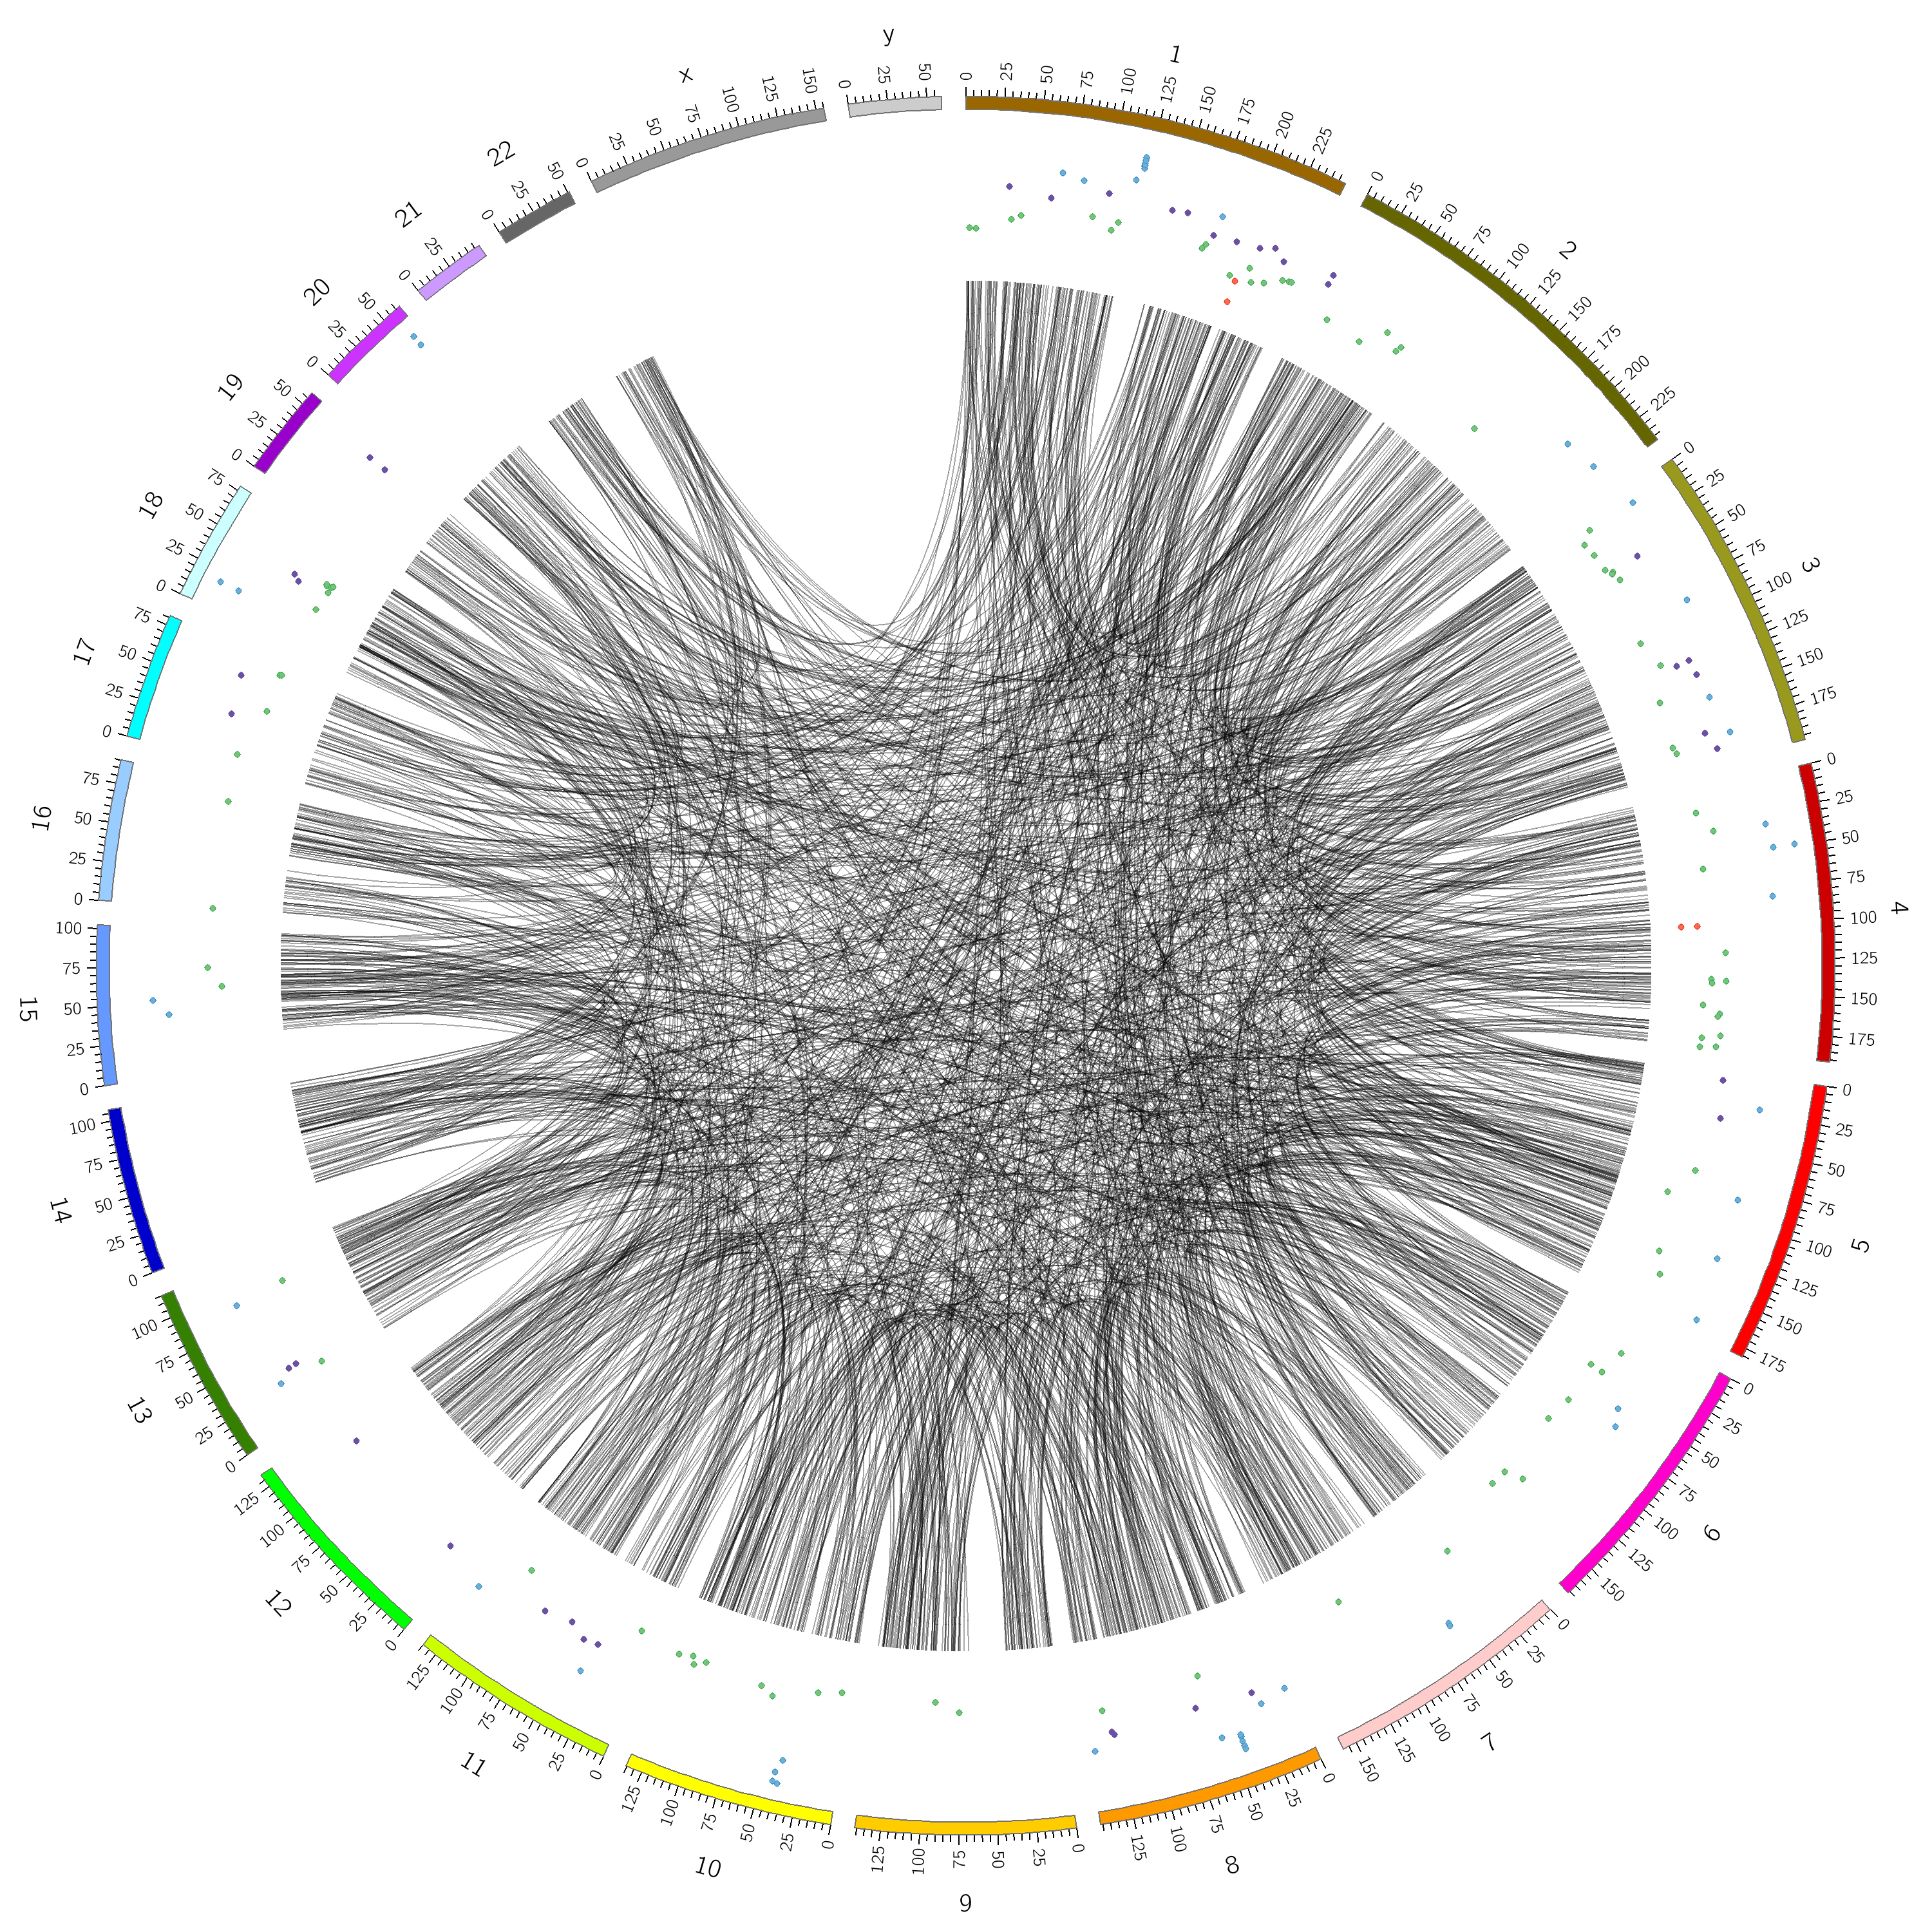
\includegraphics[keepaspectratio,width=0.5\textwidth]{./figures/circos/SRR5365000gDNA_0529} & 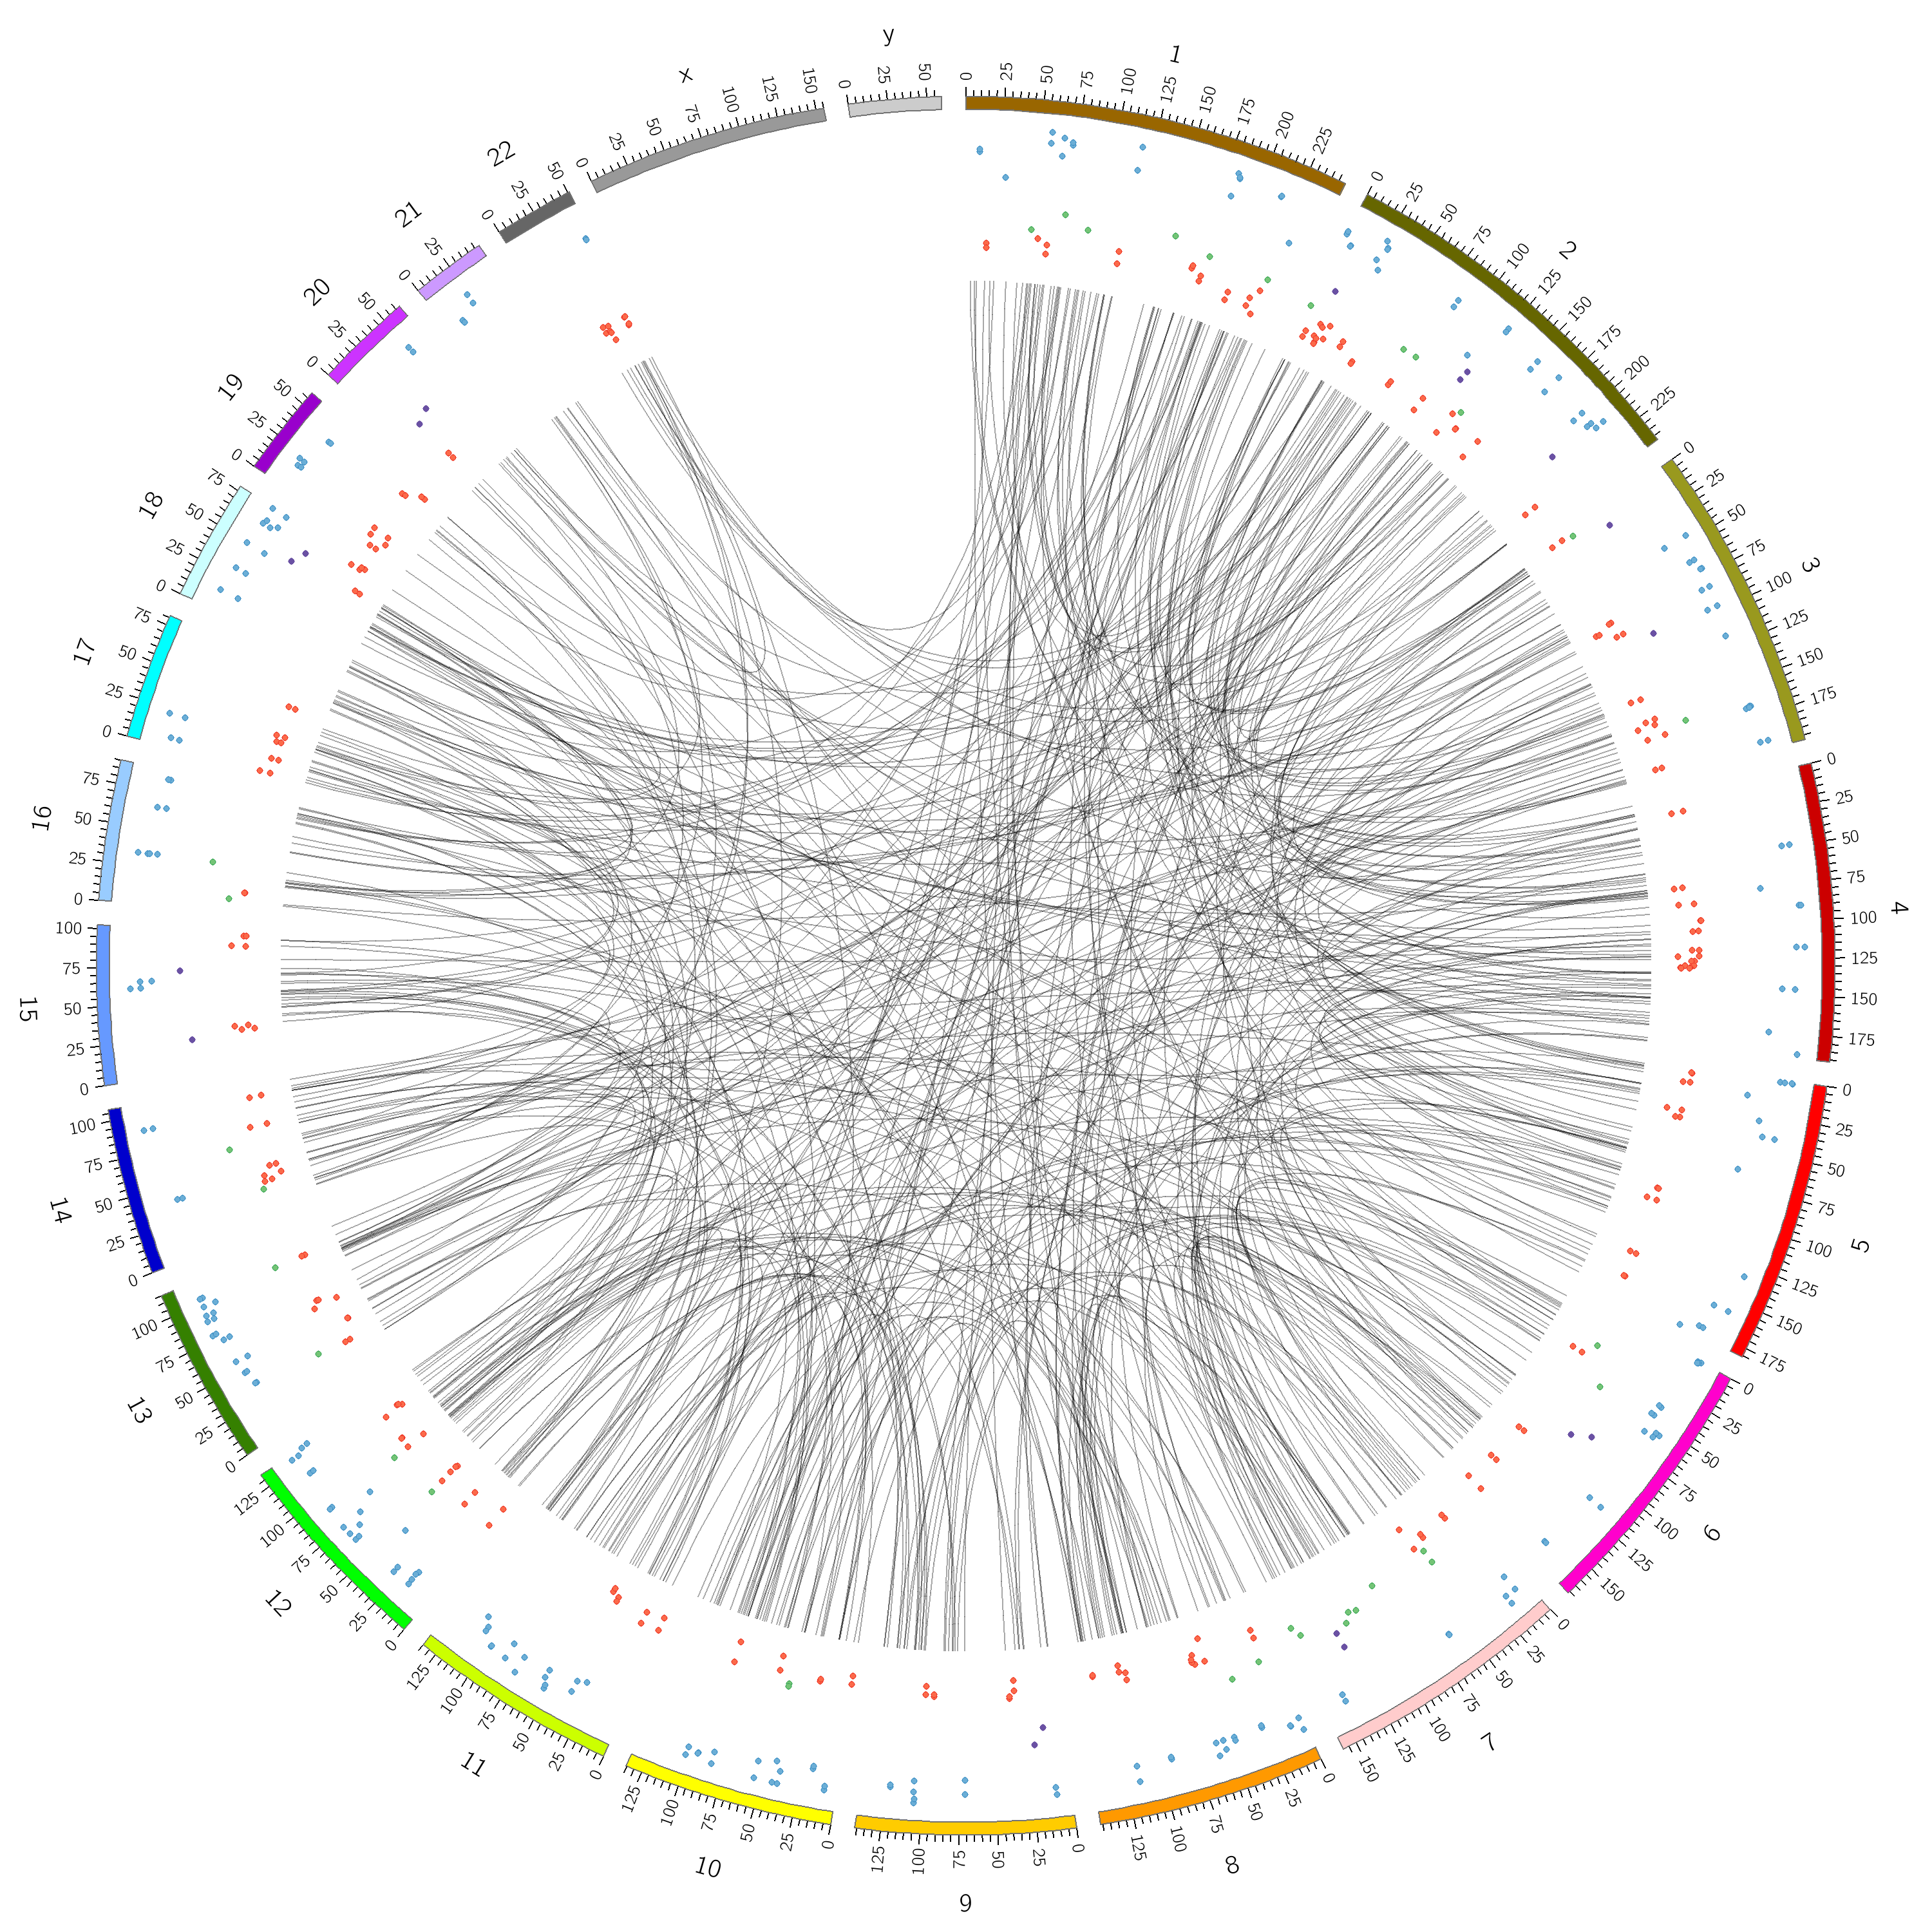
\includegraphics[keepaspectratio,width=0.5\textwidth]{./figures/circos/SRR5365374_0529} \\
\end{tabular}
\caption[Chimera breakpoints shown in Circos plots (part 2)]{Chimera breakpoints shown in Circos plots for bulk genomic DNA and single-cell samples (part 2). Cross-chromosome chimera pairs are connected, shown as black lines in the center. Inverted chimera breakpoints are represented as red dots. Inverted \& large-insert chimera breakpoints are green dots. Large-insert chimera breakpoints are purple dots. Outward chimera breakpoints are blue dots.}
\label{fig:part2_LX0gDNAcircos}
\end{figure}


In order to visualize the location of chimera discovered, I plotted all chimera pairs throughout the genome in Circos plots (Fig. \ref{fig:LX0gDNAcircos} and \ref{fig:part2_LX0gDNAcircos}) \cite{Krzywinski:2009ix}. All chimera pairs shown were based on the normalization of 430K mapped sequencing reads for each sample. Each Circos plot shows the chimera locations across the entire set of chromosomes. The VM gDNA represents the RPE bulk genomic DNA sample without any PCR enrichment, indicating that the unamplified genomic DNA contains a baseline of structural variations with respect to the reference genome. The difference in frequencies of cross-chromosome chimera between the VM gDNA and other gDNA samples probably originate from PCR enrichment and are cell-line specific. This difference shows the difficulty in benchmarking chimera performances across different studies and the importance of standardizing single-cell model systems for future technology development and characterization. 

\begin{figure}
\centering

\includegraphics[keepaspectratio,width=1\textwidth]{./figures/GenomecovLorenz}
\caption[The coverage uniformity and the genome coverage performance]{The coverage uniformity and the genome coverage performance. (a) The coverage uniformity is shown as Gini index vs amplification gain. Gini index of 1 means the maximum bias. (b) Genome coverage percentage is shown for all datasets.}
\label{fig:GenomecovLorenz}
\end{figure}

\subsection{Coverage uniformity and physical genome coverage performances}
In order to evaluate the coverage uniformity and the physical genome coverage performance of single amplified human genomes, \textit{virtual microfluidic} VM (8 cells), eWGA (5), MALBAC (2), MDA (2), LIANTI (3) were first downsampled to 1$\times$ mapped depth (about 30 million reads). Fig. \ref{fig:GenomecovLorenz}a quantifies the coverage bias vs amplification gain. The coverage bias is quantified using the area under Lorenz curve and is represented as the Gini index. Including the amplification gain is important for quantifying coverage biases, as the literature has shown MDA over-amplification results in highly biased genomes \cite{deBourcy:2014ji}. Fig. \ref{fig:GenomecovLorenz}b shows the genome coverage percentage across all samples at 1$\times$ mapping depth. \textit{Virtual microfluidic} samples show a range of performance in both coverage uniformity and physical genome coverage percentage. This is most likely due to the uneven amplification gain obtained for 8 different samples (from 28093 to 565 folds). Future experiments with amplification gain control of above 25000 fold should be able to produce much improved overall performance in the coverage uniformity and the genome coverage percentage. Overall, the LIANTI method shows superior performances in terms of coverage uniformity, physical genome coverage and chimera reduction. This new scheme of whole genome amplification might overtake MDA's dominant place in future single cell genomic applications. 

The performances of single-cell analysis are often cherry-picked and selectively reported. The Nanodrop method's high sequencing-depth data were cherry-picked based on the quality of its low-depth dataset, thus we excluded it from the coverage and uniformity comparison. It is highly likely that eWGA and LIANTI single cells are cherry-picked as the best subsets but it is not yet confirmed. The effect of cherry-picking, known as the fallacy of incomplete evidence, gives a false impression on the overall quality of single cell sequencing technologies and inflates performance measurements such as coverage uniformity and genome coverage. In contrast, the 8 VM cells were the entire dataset that went through MDA, library preparation and sequencing (without cherry picking). I believe there is a great potential in improving data qualities and \textit{virtual microfluidics} measurements represent the foremost of single-cell technology platform to this date. 

\section{Conclusion}
In conclusion, \textit{virtual microfluidics} enables high-quality single-cell genome sequencing with 1 (compared with Nanodrop) $\sim$ 8 fold (compared with eWGA) chimera rate reduction in MDA reaction while only requiring basic bench tools. It eliminates the need of creating ultra-small discrete chambers for sub-microliter MDA reactions. This chapter also showcase the importance of quantifying chimeric DNA rearrangements from single-cell genomic amplification and library preparation processes. Such study is important in providing a baseline analysis of the chimera signatures and can be used for predicting the amount of false positive DNA rearrangements that are of interests to prenatal and cancer diagnosis. \textit{Virtual microfluidics} also has a potential as a flexible platform for combining new WGA chemistry such as LIANTI and library preparation methods involving \textit{in situ} tagmentation that will push the throughput and data quality from single-cell WGA to a new level. 

\section{Materials and Methods}
\subsection{Experimental methods}
The hTERT RPE--1 (ATCC) cell line stably expressing GFP-H2B were cultured in 10\% final concentration of fetal bovine serum (FBS) and 0.01 mg\slash ml hygromycin in ATCC-formulated DMEM:F12 Medium (Catalog No. 30--2006). When the culture was at > 80\% confluence, it was serum-starved for 12 hrs overnight for cell cycle synchronization. A blank Costar 384-well plate with glass bottom was imaged for GFP fluorescence and under the white light before cell deposition. Cells were trypsinized, counted and diluted to 1 cell\slash $\mu$l, and 1 $\mu$l was added to each well of the 384 plate. The plate was spin down briefly and imaged for GFP fluorescence and under white light to confirm single-cell occupancy in each well. To the wells with single cells, 4 $\mu$l of lysis buffer (30 mM Tris-HCl, 10 mM NaCl, 5 mM EDTA, 0.5\% Triton X--100 and 1 mg\slash ml proteinase K) with hexamer of final concentration 50 $\mu$M was added and heated at 50 $^{\circ}$C for 3 hrs and at 70 $^{\circ}$C for 30 mins to denature proteinase. Then the plate was heated at 98 $^{\circ}$C for 4 mins and at 95 $^{\circ}$C for 2 mins to ensure proper fragmentation based on eWGA paper. Finally, DNA denaturation happened at 95 $^{\circ}$C for 5 mins, and the plate was cold quenched on ice for 20 mins. 

After cold quenching, PEG hydrogel reaction mix was added to the well. Gels were formed in 20 mins at room temperature and maintain at 30 $^{\circ}$C for 12 hrs for MDA reaction and 65 $^{\circ}$C for 5 mins to deactivate $\Phi$29. Reaction wells were imaged with SYTOX orange DNA intercalating dye. To retrieve DNA for library preparation, 6.6 $\mu$l of 400 mM KOH was added to incubate for 10 mins at 72 $^{\circ}$C and 3 $\mu$l 3.75\% acetic acid neutralization buffer was added. The neutralized gel-DNA mix was SPRI cleaned with 1X:1X volume ratio and library prepared with standard Nextera procedures with 12 cycles of PCR. The 8 cell libraries were loaded on HiSeq 2500 in the rapid run mode. 

The experimental difference from \textit{virtual microfluidics} on the microbial sample is that we diluted single cells and Poisson loaded them into 384 wells. A single genome was fragmented, evenly distributed in the PEG hydrogel and went through digital MDA. Only one round of MDA was conducted. 

\subsection{Bioinformatic methods}

Raw sequencing fastq.gz files were quality and adapter trimmed using Trimmomatic. For fast processing of chimera analysis, fastq files were downsampled to 600,000 reads using Seqtk (https:\slash \slash github.com\slash lh3\slash seqtk with seed 100). Fastq files were mapped with BWA under default mode both pair-ended and single-ended. BAM files were sorted by mapping coordinates. Mark PCR and optical duplicates, and mask repeat region with the file downloaded from UCSC Genome Browser (assembly:GRCh37\slash hg19, group: Repeats, track: RepeatMasker, output:BED). The mapping statistics were retrieved from BAM files using gaemr get\_simple\_bam\_stats.py, and all BAM files were downsampled based the BAM stats resulting to 430,000 reads each sample ---both forward and reverse reads. Single-ended mapped BAM files were sorted by query names and merged (Fig. \ref{fig:Chimera_Mapping}). 

Genome coverage was obtained using Bedtools genomecov. Lorenz curves were obtained by first processing BAM files (duplicates marked) using SAMtools mpileup and then ranking the ascending coverage per base pair (see Fig. \ref{fig:ESDataAnalysis} in Chapter 3 for detail). 

\begin{figure}
\centering
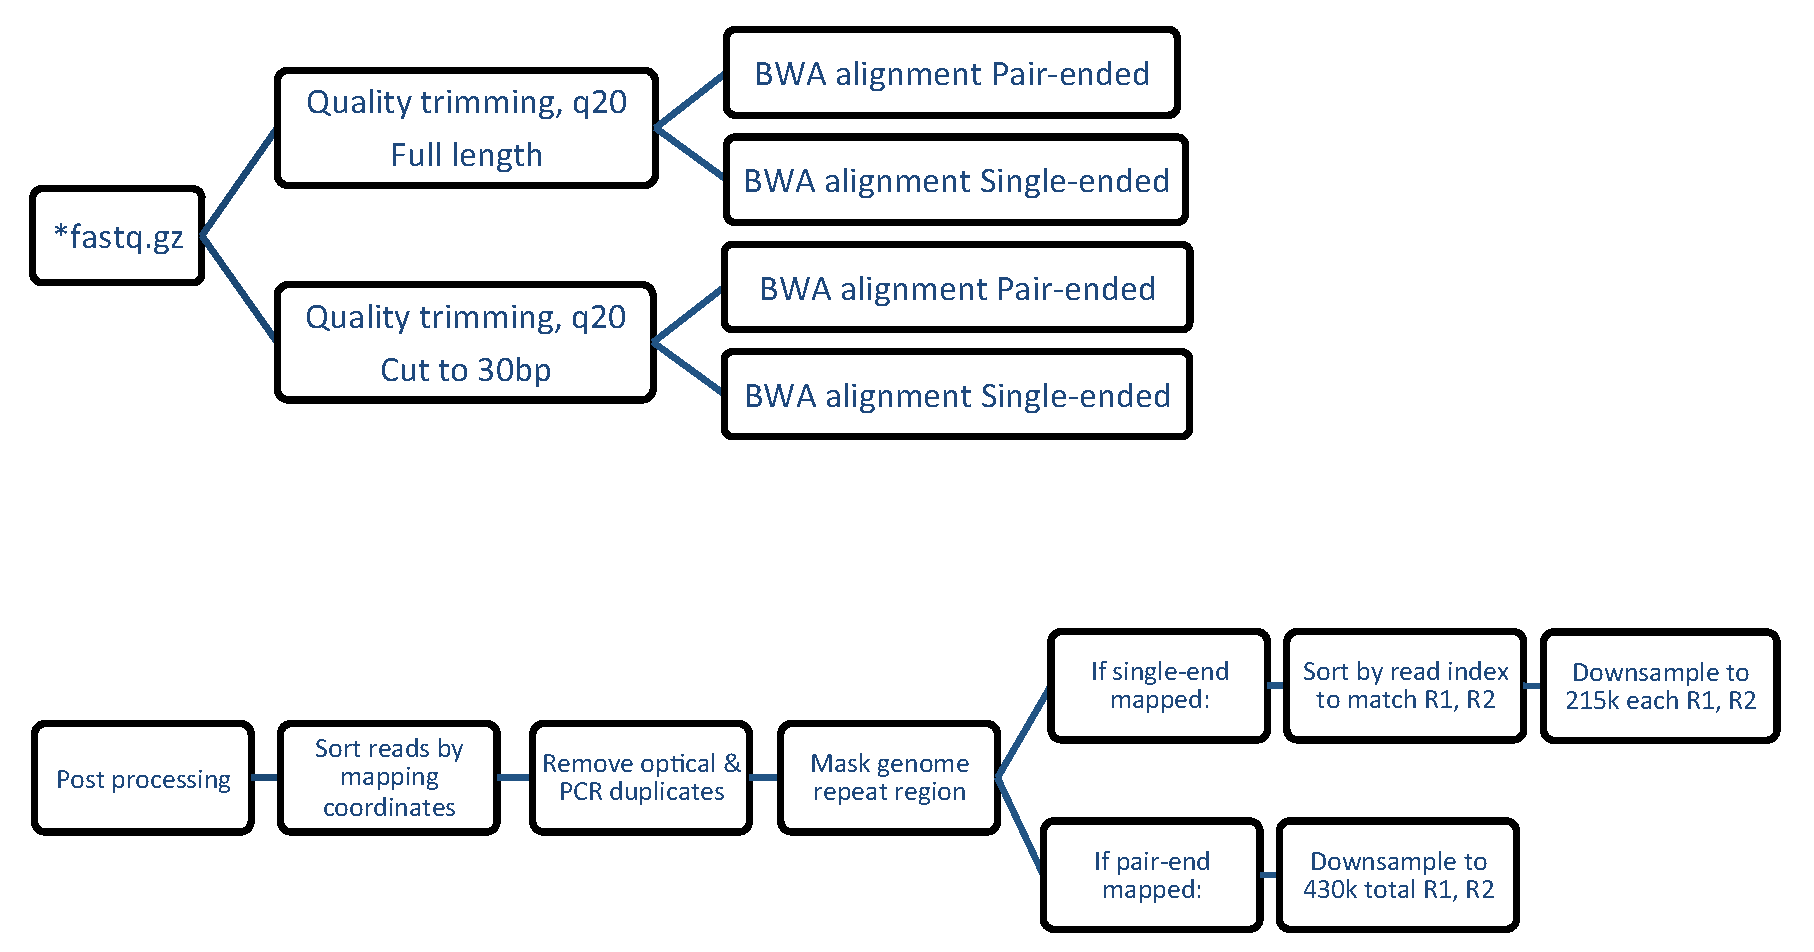
\includegraphics[keepaspectratio,width=\textwidth]{./figures/Chimera_Mapping}
\caption[Bioinformatic workflow for chimera analysis]{Bioinformatic workflow for chimera analysis.}
\label{fig:Chimera_Mapping}
\end{figure}

% Supplementary Text:
% Long-range sequencing technology:
% Recent developments in long-read sequencing, such as PacBio and Nanopore systems, have enabled the detection of chimera in human genome assembly previously made through Illumina short-read data \cite{Pendleton:2015jp}. Long-range sequencing can potentially reduce the amount of chimeric artifacts from PCR-based sequencing library preparation and requires multiple passes of sequencing materials, which is challenging without whole genome amplification.

% One category of TE is called retrotransposon L1, which duplicates through RNA intermediates and reverse transcribes to insert at new genomic locations \cite{Cordaux:2009bb}. L1 has been associated with insertional mutagenesis and is a potential source of genotypic variation among neurons \cite{Evrony:2012dl}. 